%%%%%%%%%%%%%%%%%%%%%%%% Springer-Verlag
\documentclass[epjST,usenames,dvipsnames,vecphys]{svjour}

\usepackage{amsmath,amssymb}
\usepackage{float}
\usepackage{hyperref}
\usepackage[framemethod=TikZ]{mdframed}
\usepackage{footnote}
%\usepackage{natbib}
\usepackage{doi}
\usepackage{enumitem}

\makesavenoteenv{tabular}
\makesavenoteenv{table}
\makesavenoteenv{figure}
%\makesavenoteenv{mdframed}
%\usepackage[usenames,dvipsnames]{xcolor}
\usepackage{xcolor}
\usepackage{graphicx}
%\usepackage{graphics}

% Useful macros for equations and units
\newcommand*{\TeV}{\text{ TeV}}
\newcommand*{\GeV}{\text{ GeV}}
\newcommand*{\MeV}{\text{ MeV}}
\newcommand*{\keV}{\text{ keV}}
\newcommand*{\eV}{\text{ eV}}
\newcommand*{\meV}{\text{ meV}}
\newcommand*{\Msun}{\mathrm{M}_{\odot}}
\newcommand*{\bb}{\boldsymbol}
\newcommand*{\beqn}{\begin{equation}}
\newcommand*{\eeqn}{\end{equation}}
\newcommand{\req}[1]{Eq.~(\ref{#1})}
\newcommand{\rf}[1]{Fig.~{\ref{#1}}}
\newcommand{\rt}[1]{Table~{\ref{#1}}}
\newcommand{\rsec}[1]{Sec.~{\ref{#1}}}
\newcommand{\rchap}[1]{Ch.~{\ref{#1}}}
\newcommand{\rapp}[1]{Appendix~{\ref{#1}}}
\newcommand{\mydoi}[2]{\href{http://dx.doi.org/#2}{#1}}
\newcommand{\E}{\mathrm{e}}
\newcommand{\ie}{{\em i.e.}} % i.e.
\newcommand{\ms}[1]{\rule[-#1mm]{0mm}{0mm}}

% Struts for tables 
\newcommand\Tstrut{\rule{0pt}{2.6ex}}
\newcommand\Bstrut{\rule[-0.9ex]{0pt}{0pt}}
\newcommand{\TBstrut}{\Tstrut\Bstrut}
  
\begin{document}
%%%%%%%%%%%%%%%%%%%%%%%%
% This WON'T just be single files!
% Temporary structure!
\title{Particles and Plasma in\\ 
 Cosmological Evolution}

\author{
Jeremiah Birrell\inst{1}, %\inst{1}\fnmsep\thanks{\email{jeremey.birrell@gmail.com}},
Christopher Grayson\inst{1}, %\inst{1}\fnmsep\thanks{\email{chrisgray1044@arizona.edu}},
Johann Rafelski\inst{1}, %\inst{1}\fnmsep\thanks{\email{johannr@arizona.edu}}
\newline Andrew Steinmetz\inst{1}\fnmsep\thanks{Corresponding author \email{ajsteinmetz@arizona.edu}}, 
Cheng Tao Yang\inst{1}%\fnmsep\thanks{\email{chengtaoyang@arizona.edu}}
}

\institute{Department of Physics, The University of Arizona, Tucson, AZ, 85721, USA
}

\abstract{
We aim to deepen the understanding of the primordial composition of the Universe in the temperature range $300\,\mathrm{MeV}>T>0.02\,\mathrm{MeV}$. Within the Big Bang model, the Universe began as a highly energetic fireball with an immensely high temperature and energy density. Consequently, an ultra-relativistic plasma was generated whose content of fundamental particles (such as quarks, leptons, and gauge bosons) dynamically changed as the Universe expanded and cooled. These elementary particles were abundantly present once the temperature dropped below $T=130$\,~GeV. At $T=\mathcal{O}(1)$\,~MeV through the free-streaming era up to today, we characterize the deviation of the neutrino spectrum from equilibrium and in particular we demonstrate the presence of chemical non-equilibrium that continues to the present day. We focus on the distinction between chemical and kinetic equilibrium and freeze-out. Using these concepts, we derive those properties of neutrino freeze-out that depend only on conservation laws and are independent of the details of the microscopic scattering processes. We characterize the dependence of both $N_\nu$ and the deviation of the neutrino distribution from chemical equilibrium on the neutrino kinetic freeze-out temperature. We detail a spectral method was designed extend the regime of applicability to systems far from chemical equilibrium and/or that undergo significant reheating. In the early universe during the hot dense electron-positron plasma epoch (after neutrino freeze-out), we analyze the paramagnetic characteristics of electron-positron plasma when exposed to an external primordial field. We note the high density of antimatter in the form of positrons which persisted into the Big Bang Nucleosynthesis era.
} 
\maketitle
\section{Introduction}
\label{sec:Intro}
\section*{Context}
\label{sec:context}
This review collects in edited and resequenced manner the contents of four recent Ph.D. Thesis completed at the Department of Physics, The University of Arizona by: Jeremiah Birrell~\cite{BirrellThesis:2014}, Christopher M. Grayson~\cite{GraysonThesis:2024}, Andrew J. Steinmetz~\cite{SteinmetzThesis:2023}, and Cheng Tao Yang~\cite{YangThesis:2023}. We include material incorporated to the thesis in published form as well as further going related work which due to time constraints did not find its way to the formal thesis document.

\setcounter{tocdepth}{2}
\tableofcontents

%%%%%%%%%%%%%%%%%%%%%%%%%%%%%%%%%%%%%%%
\section{Cosmology introduction}
\label{sec:flrw}
%%%%%%%%%%%%%%%%%%%%%%%%%%%%%%%%%%%%%%%
\noindent This section introduces some necessary concepts which will be useful in describing the magnetization of the electron-positron primordial plasma in \rchap{chap:cosmo}. We operate under the $\Lambda$ Cold Dark Matter $(\Lambda\mathrm{CDM})$ model of cosmology where the contemporary universe is approximately 69\% dark energy, 26\% dark matter, 5\% baryons, and $<1$\% photons and neutrinos in energy density~\cite{Davis:2003ad,Planck:2018vyg}. The standard picture of the universe's evolution is outlined in \rf{fig:cosmo}.

The Friedmann-Lema{\^i}tre-Robertson-Walker (FLRW) line element and metric~\cite{weinberg1972gravitation} in spherical coordinates is
\begin{gather}
    \label{FLRW} ds^2=dt^2-a^2(t)\left[\frac{dr^2}{1-kr^{2}}+r^{2}d\theta^2+r^{2}\sin\theta^{2}d\phi^2\right]\,,\\
    g_{\alpha\beta}=
    \begin{pmatrix}
        1&0&0&0\\
        0&-\frac{a^{2}(t)}{1-kr^{2}}&0&0\\
        0&0&-a^{2}(t)r^{2}&0\\
        0&0&0&-a^{2}(t)r^{2}\sin\theta^{2}
    \end{pmatrix}\,.
\end{gather}
The Gaussian curvature $k$ informs the spatial shape of the universe with the following possibilities: infinite flat Euclidean $(k=0)$, finite spherical but unbounded $(k=+1)$, or infinite hyperbolic saddle-shaped $(k=-1)$. Observation indicates our universe is flat or nearly so.

%%%%%%%%%%%%%%%%%%%%%%%%%%%%%%%%%%%%%%%
\begin{figure}[ht]
 \centering
 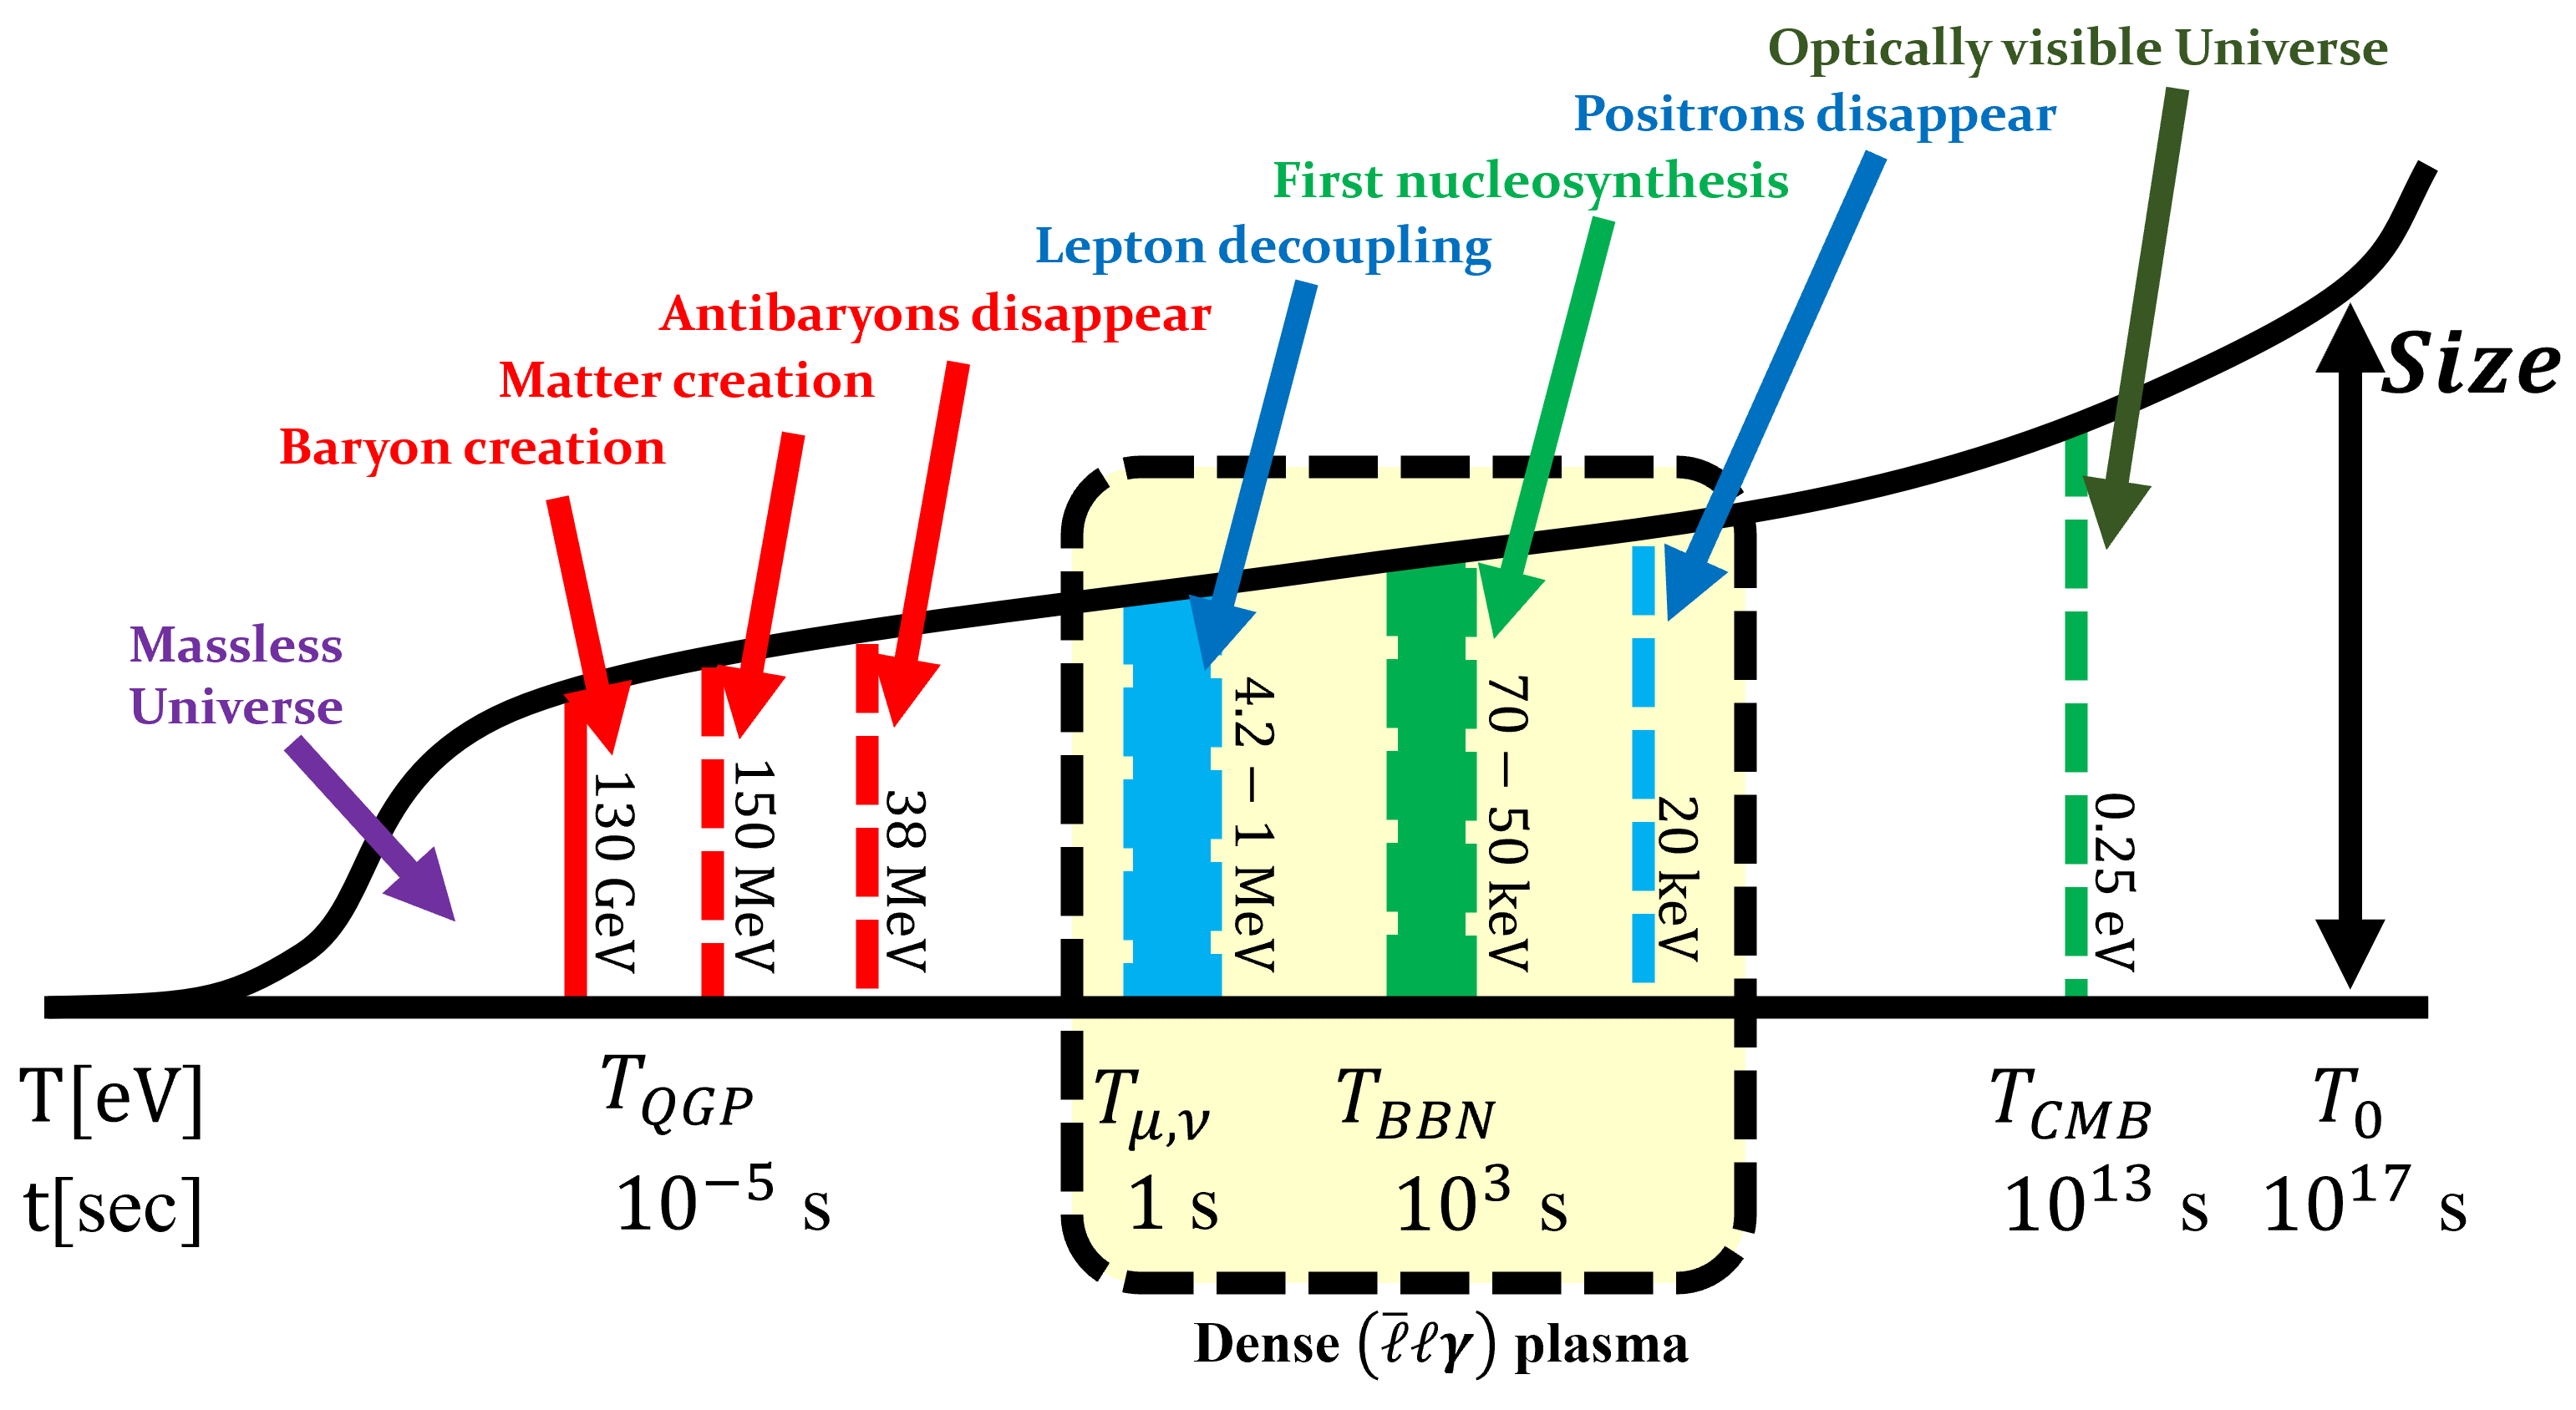
\includegraphics[width=0.95\linewidth]{plots/chap01intro/thesis_universe.png}
 \caption{A schematic of the universe's evolution since the Big Bang. The region of interest studied in this dissertation is emphasized (in the highlighted box) to contain a dense nearly charge neutral matter-antimatter plasma.}
 \label{fig:cosmo} 
\end{figure}
%%%%%%%%%%%%%%%%%%%%%%%%%%%%%%%%%%%%%%%

The scale factor $a(t)$ denotes the change of proper distances $L(t)$ over time as
\begin{gather}
    L(t)=L_{0}\frac{a_{0}}{a(t)}\rightarrow L(z)=L_{0}(1+z)\,,
\end{gather}
where $z$ is the redshift and $L_{0}$ the comoving length. In an expanding (or contracting) universe which is both homogeneous and isotropic. This implies volumes change with $V(t)=V_{0}/a^{3}(t)$ where $V_{0}=L_{0}^{3}$ is the comoving Cartesian volume. The evolutionary expansion of the universe is then traditionally defined in terms of the Hubble parameter $H(t)$ following the conventions in~\cite{weinberg1972gravitation}
\begin{gather}
  \label{Friedmann:1} H(t)^{2}\equiv\left(\frac{\dot a}{a}\right)^2=\frac{8\pi G_{N}}{3}\rho_\mathrm{total},\qquad \rho_\mathrm{total}(t)=\rho_{\Lambda}+\rho_\mathrm{DM}(t)+\rho_\mathrm{Baryons}(t)+\ldots\\
  \label{Friedmann:2}
  \frac{\ddot a}{a}=-qH^2,\qquad 
q\equiv -\frac{a\ddot a}{\dot a^2},\qquad \dot H=-H^2(1+q).
\end{gather}
where $G_N$ is the Newtonian constant of gravitation. \req{Friedmann:1} and \req{Friedmann:2} are also known as the Friedmann equations. The total density $\rho_\mathrm{total}$ is the sum of all contributions from any form of matter, radiation or field. This includes but is not limited to: dark energy $(\Lambda)$, dark matter (DM), baryons (B), leptons $(\ell,\nu)$ and photons $(\gamma)$. Depending on the age of the universe, the relative importance of each group changes as each dilutes differently under expansion with dark energy infamously remaining constant in density and accelerating the universe today.

The parameter $q$ is the cosmic deceleration which for historical reasons is positive $q>0$ under deceleration. This convention was chosen before the discovery of dark energy under the tacit assumption that the universe would be decelerating. The value of $q$ depends on energy content: The early universe was radiation dominated $(q = 1)$, subsequently matter dominated $(q = 1/2)$, and lastly the contemporary universe is undergoing a transition from matter to dark energy dominated approaching the asymptotic value of $q = -1$; see~\cite{Rafelski:2013yka}.

We can consider the expansion to be an adiabatic process~\cite{Abdalla:2022yfr} which results in a smooth shifting of the relevant dynamical quantities. As the universe undergoes isotropic expansion, the temperature decreases as 
\begin{gather}
 \label{tscale}
 T(t)=T_{0}\frac{a_{0}}{a(t)}\rightarrow T(z)=T_{0}(1+z)\,,
\end{gather}
where $z$ is the redshift. The entropy within a comoving volume is kept constant until gravitational collapse effects become relevant. The comoving temperature $T_{0}$ is given by the the present CMB temperature $T_{0}=2.7{\rm\ K}\simeq2.3\times10^{-4}\eV$~\cite{Planck:2018vyg}, with contemporary scale factor $a_{0}=1$.

As the universe expands, redshift reduces the momenta of particles lowering their contribution to the energy content of the universe. This cosmic redshift is written as
\begin{alignat}{1}
  \label{Redshift} p_{i}(t) = p_{i,0}\frac{a_{0}}{a(t)}\,.
\end{alignat}
Momentum (and the energy of massless particles $E=pc$) scales with the same factor as temperature. The energy of massive free particles in the universe however scales differently based on their momentum (and thus temperature).

When hot and relativistic, particle energy decreases inversely with scale factor like radiation. As the particles transition to non-relativistic (NR) energies, they decrease with the inverse square of the scale factor
\begin{alignat}{1}
    \label{EScale} E(t) = E_{0}\frac{a_{0}}{a(t)}\xrightarrow{\mathrm{NR}}\  E_{0}\frac{a_{0}^{2}}{a(t)^{2}}\,.
\end{alignat}
This occurs because of the functional dependence of energy on momentum in the relativistic $E\sim p$ versus non-relativistic $E\sim p^{2}$ cases.

\subsection{The standard FLRW-Universe model}
%In this section we will focus on the following:
%\begin{itemize}
%    \item The Robertson –Walker Universe
%    \item The Friedmann equation (Hubble %    \item The composition of the universe
%\end{itemize}
The Friedmann-Lemaitre-Robertson-Walker (FLRW) Universe is a theoretical model used widely to describe the cosmological evolution of the Universe. It is based on the cosmological principles which assumes homogeneity and isotropy of the Universe on large scales. In general, the FLRW metric can be written as
\begin{align}\label{metric}
ds^2=c^2dt^2-a^2(t)\left[ \frac{dr^2}{1-kr^2}+r^2(d\theta^2+\sin^2\theta\,d\phi^2)\right].
\end{align}
The metric is characterized by the scale factor $a(t)$ which measures the size of the Universe as a function of time $t$. The geometric parameter $k$ identifies the Gaussian geometry of the spatial hyper-surfaces defined by co-moving observers. The metrics are qualitatively different depending on the value of $k$. We have $k=1$ which correspond to the closed Universe,  $k=0$ correspond to flat Universe, and $k=-1$ for open geometries of the Universe. Current observation of cosmic microwave background (CMB) anisotropy preferred value $k=0$~[\cite{Planck:2013pxb,Planck:2015fie,Planck:2018vyg}].


The cosmological equations that describe the evolution of the Universe are derived from the Einstein equations. In general, the Einstein equation with cosmological constant $\Lambda$ can be written as:
\begin{equation}\label{Einstein}
  G^{\mu\nu}=R^{\mu\nu}-\left(\frac R 2 +\Lambda\right) g^{\mu\nu}=8\pi G_N T^{\mu\nu}, 
\quad R= g_{\mu\nu}R^{\mu\nu}.  
\end{equation}
where $G_{N}$ is the Newtonian gravitational constant, and $T^{\mu\nu}$ is the stress-energy tensor. Given the homogeneous and isotropic symmetry conditions imply that the matter context of the Universe can be expressed as a perfect fluid. The stress-energy tensor $T^\mu_\nu$ of perfect fluid can be written as
\begin{align}
 T^\mu_\nu =\mathrm{diag}(\rho, -P, -P, -P).
\end{align}
where $\rho$ is energy density and an $P$ is the isotropic pressure.

Substituting the perfect fluid form of the stress-energy tensor into the Einstein equations, one can derive the cosmological equations that describe the evolution of the Universe. We then obtain Friedmann equations as follows:
\begin{align}
\label{Hubble} 
&H^{2}\equiv\left(\frac{\dot a}{a}\right)^2=\frac{8\pi G_{N}}{3}\rho-\frac{k}{a^2}+\frac{\Lambda}{3},\\
\label{q_value}
&qH^2=\frac{4\pi G_{N}}{3}\left(\rho+3P\right)-\frac{\Lambda}{3},\qquad q\equiv -\frac{a\ddot a}{\dot a^2},
\end{align}
where $H$ is the Hubble parameter,  $q$ is the deceleration parameter. These equations relate the dynamics of the scale factor $a(t)$ to the energy density and pressure of the cosmic plasma. On the other hand, considering the divergence freedom of the total stress-energy tensor $\nabla_\nu T^{\mu\nu}=0$. For $\mu=0$ component, we have
\begin{align}\label{energy_eq}
\nabla_\nu T^{0\nu}=\frac{d\rho}{dt}+3H(\rho+P)=0
\end{align}
which provides dynamical evolution equation for $\rho(t)$ and $P(t)$. Solutions of Eq.~(\ref{energy_eq}) describes the time evolution of  energy density and pressures in the Universe. Given the energy density and pressure as a function of time, we can illustrates how the Universe evolves according to the Friedmann equations Eq.~(\ref{Hubble}) and Eq.~(\ref{q_value}). Solving these equations allows us to understand the dynamics and evolution of the Universe such as the Hubble expansion and the behavior of matter and energy over cosmic time.

\subsection{Cosmic plasma in early Universe $300\,\mathrm{MeV}>T>0.02\,\mathrm{MeV}$}
%In this section we will focus on the following:
%\begin{itemize}
%    \item Five different plasma epoch from $0.3\mathrm{GeV}>T>20$keV
%\end{itemize}

The primordial hot Universe fireball underwent several practically adiabatic phase changes that dramatically evolved its bulk properties as it expanded and cooled~[\cite{Rafelski:2023emw}]. We present an overview of the Universe evolution as a function of temperature from $300\,\mathrm{MeV}>T>0.02\,\mathrm{MeV}$ and main events constituting the history of the early Universe in Fig.~\ref{Overview_fig}. After the electroweak symmetry breaking epoch and presumably inflation, the comic plasma in the early Universe evolves in the following sequence:

%%%%%%%%%%%%%%%%%%%%%%%%%%%%%%%%%%%%%%%
\begin{figure}[ht]
 \centerline{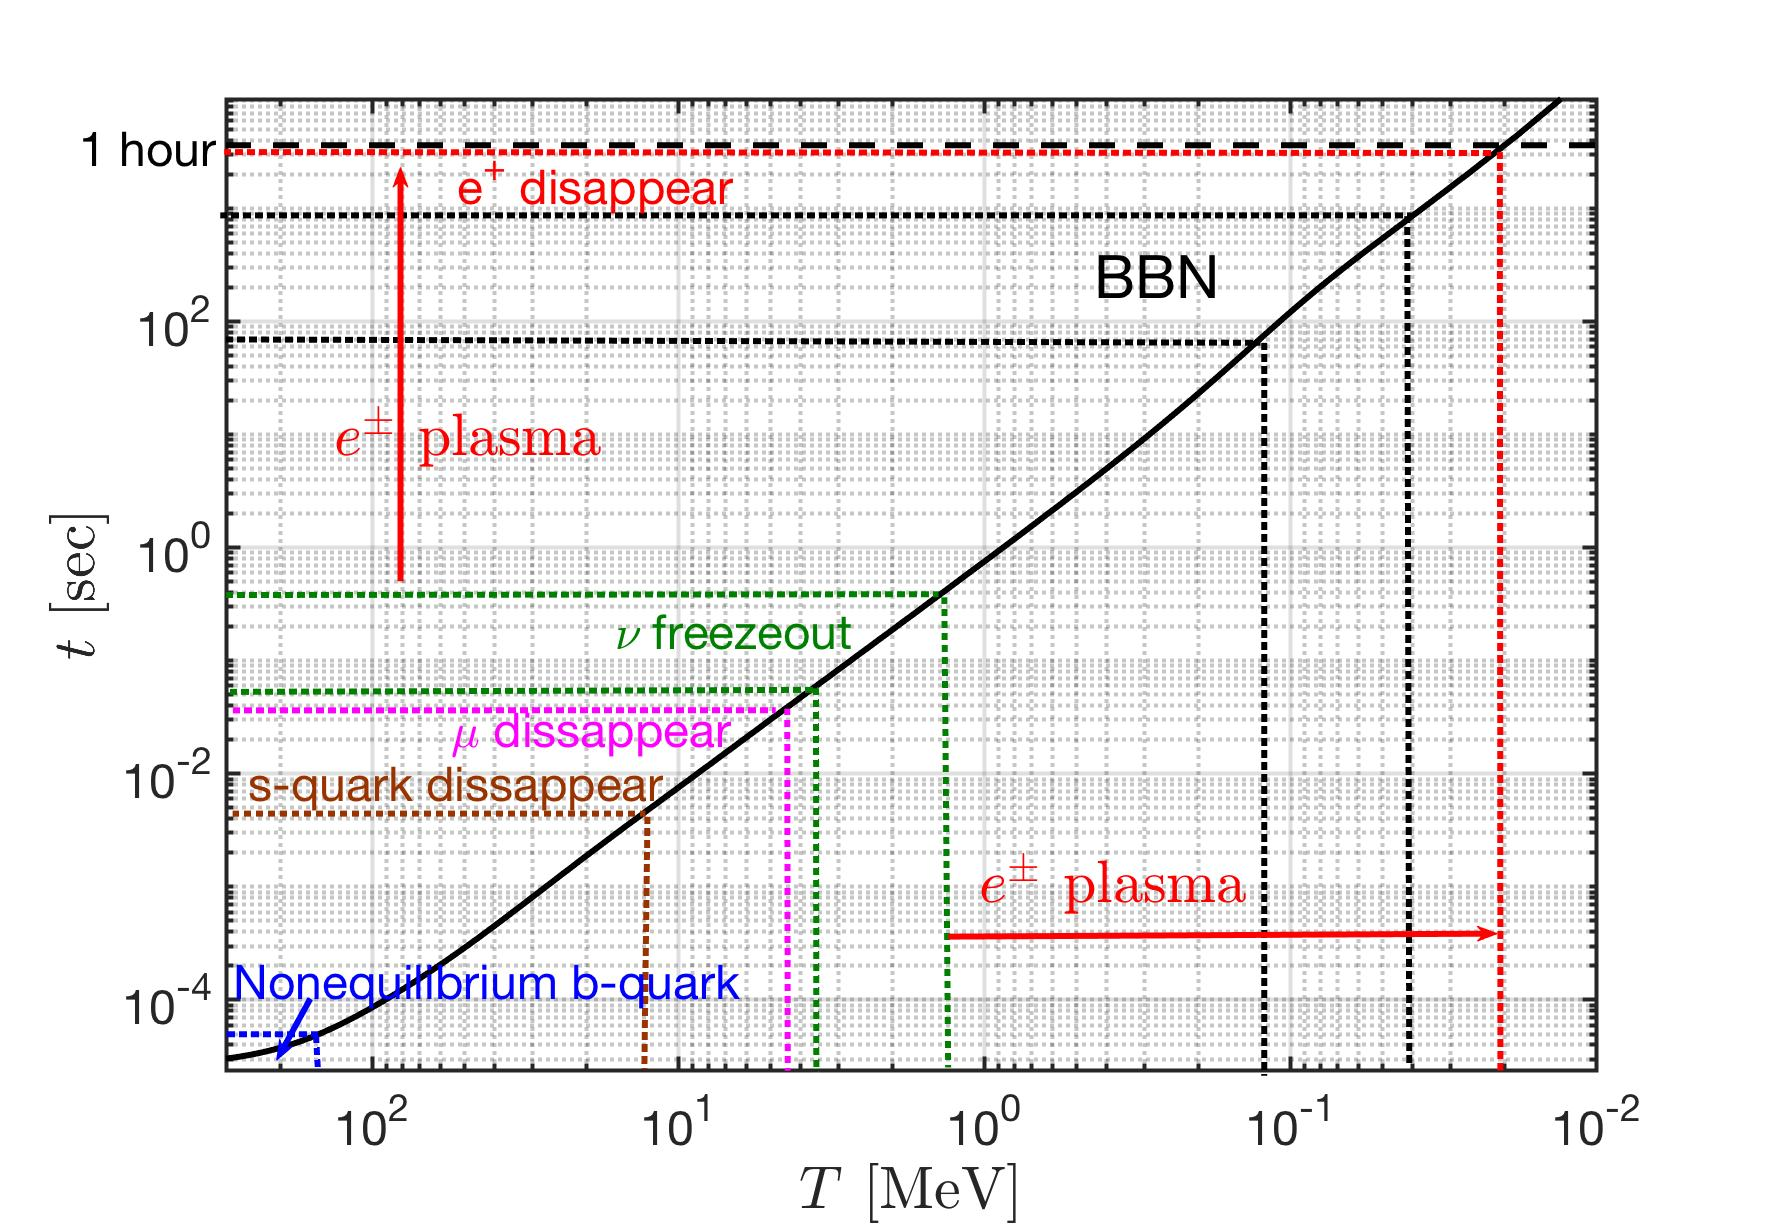
\includegraphics[width=\textwidth,width=\linewidth]{./plots/CosmicTimeTemperature_Project}}
 \caption{The time evolution of the early Universe as a function of temperature from $300\,\mathrm{MeV}>T>0.02\,\mathrm{MeV}$ and 
 different sequence of main events are shown with the temperature/time range in the evolution. }
 \label{Overview_fig}
\end{figure}
%%%%%%%%%%%%%%%%%%%%%%%%%%%%%%%%%%%%%%%

\begin{enumerate}
    \item \textbf{Primordial quark-gluon plasma}: 
    At early times when the temperature was between $130\,\mathrm{GeV}>T>0.15\,\mathrm{GeV}$ we have the building blocks of the Universe as we know them today, including the leptons, vector bosons, and all three families of deconfined quarks and gluons which propagated freely in plasma. As all hadrons are dissolved into their constituents during this time, strongly interacting particles $u,d,s,t,b,c,g$ controlled the fate of the Universe. When temperature is near to the QGP phase transition $300\, \mathrm{MeV}>T>150$ MeV, the bottom quark  breaks the detail balance and disappearance from particle inventory provides the arrow in time (see Chapter~\ref{Bottom} for detail).
    
    \item \textbf{Hadronic epoch}: Around the hadronization temperature $T_H\approx150\,\mathrm{MeV}$, a phase transformation occurred, forcing 
    the free quarks and gluons become confined within baryon and mesons [\cite{Letessier:2005qe}]. In the temperature range $ 150\,\mathrm{MeV}>T>20\,\mathrm{MeV}$, the Universe is rich in physics phenomena involving strange mesons and (anti)baryons including (anti)hyperon abundances~[\cite{Fromerth:2012fe,Yang:2021bko}]. The antibaryons disappear from the Universe at temperature $T=38.2$ MeV, and strangeness can be produced by the inverse decay reactions that are in equilibrium via weak, electromagnetic, and strong interactions in the early Universe until $T\approx13$ MeV (see Chapter~\ref{Strangeness} for detailed discussion).

    
    \item \textbf{Lepton-photon epoch}: For temperature $10\,\mathrm{MeV}>T>2\,\mathrm{MeV}$, the Universe contained relativistic electrons, positrons, photons, and three species of (anti)neutrinos. During this epoch massless leptons and photons controlled the fate of the Universe. Massive $\tau^\pm$ disappear from the plasma at high temperature via decay processes. However $\mu^\pm$ leptons can persist in the early Universe until temperature $T=4.2$ MeV, and positron $e^+$ can persist until the temperature $T=0.02$ MeV (See Chapter~\ref{Electron} for discussion).
    Neutrinos were still coupled to the charged leptons via the weak interaction~[\cite{Birrell:2012gg,Birrell:2014ona}] and freeze-out at temperature range $3\,\mathrm{MeV}>T>2\,\mathrm{MeV}$ which depends on the neutrino's flavors and the magnitude of the Standard Model parameters (See Chapter~\ref{Neutrino} for details). After neutrino freeze-out, they still play a important role in the Universe expansion via the effective number of neutrinos $N_{\nu}^{\mathrm{eff}}$ and affects the Hubble parameter significantly.  
    
    \item \textbf{Electron-positron epoch}: After neutrinos freeze-out at $T=3\sim2\,\mathrm{MeV}$ and become free-streaming in the early Universe, the cosmic plasma was dominated by electrons, positrons, and photons. The $e^\pm$ plasma existed until $T\approx0.02\,\mathrm{MeV}$ such that BBN occurred within a rich electron-positron plasma, and the dense number density of electron/positron also provide the opportunities to investigate magnetization process (See Chapter~\ref{Electron} for detailed discussion). This is the last time the Universe will contain a significant fraction of its content in antimatter.
\end{enumerate}
After $e^\pm$ annihilation, the Universe was still opaque to photons at this point and remained so until the recombination period at $T\approx0.25\,\mathrm{eV}$ starting the era of observational cosmology with the Cosmic Microwave Background. This period has been studied in detail before in~[\cite{Planck:2018vyg}]. Therefore, we focus on the temperature $300\,\mathrm{MeV}>T>0.02\,\mathrm{MeV}$ which corresponds to the first hour of the Universe evolution. We will address the cosmic plasma as follow: In Chapter~\ref{Bottom}, we discuss the heavy quarks (bottom/charm) abundance near to the QGP hadronization and show the nonequilibrium of bottom quark.  In Chapter~\ref{Strangeness} we study the strangeness abundance after hadronization and show the long lasting strangeness in the early Universe. In Chapter~\ref{Neutrino} we focus on the neutrino-matter interactions and the evolution of cosmic neutrino in early universe before/after freeze-out. In Chapter~\ref{Electron} we study the abundance of charged leptons $\mu^\pm$ and $e^\pm$ and show that the present of $e^\pm$ plasma plays an important role in early Universe. In Chapter~\ref{Outlook} we address the ongoing and prospective research projects for future publication.
Finally in Chapter~\ref{Summary} we summarize the important results of our study and conclusion.

\section{Introduction to Cosmology and the Relic Neutrino Background}\label{ch:intro}
At a temperature of $5$ MeV the Universe consisted of a plasma of $e^\pm$, photons, and neutrinos. At around $1$ MeV neutrinos stop interacting, or freeze-out, and begin to free-stream through the Universe. Today they comprise the relic neutrino background. Photons freeze-out around $0.25$ eV and today they make up the Cosmic Microwave Background (CMB), currently at $T_{\gamma,0}=0.235$ meV.  Relic neutrinos have not been directly measured, but their impact on the speed of expansion of the Universe is imprinted on the CMB.  Indirect measurements of the relic neutrino background, such as by the Planck satellite \cite{Planck},  constrain neutrino properties such as mass and number of massless degrees of freedom.

 In later chapters, we will study the details of the neutrino freeze-out process and their impact on observables in detail but first we present an overview of cosmology, from just prior to neutrino freeze-out until today, putting the relic neutrinos in their proper context. Much of this material, including most figures, was adapted from our paper \cite{ErasOfUniverse}.


\subsection{Standard Cosmology}\label{cosmo}
 To follow the history of the relic neutrino distribution, one must first understand the relation between the expansion dynamics of the Universe, its energy content, and the connection to the photon and neutrino temperature. For this purpose we need some preparation in the  Friedmann$-$Lemaitre$-$Robertson$-$Walker (FRW) cosmological  model, see for example \cite{hartle2003gravity,hobson,misner1973gravitation}. Assuming a homogeneous, isotropic Universe, one arrives at the spacetime metric
\beqn\label{metric}
ds^2=dt^2-a^2(t)\left[ \frac{dr^2}{1-kr^2}+r^2(d\theta^2+\sin^2(\theta)d\phi^2)\right]
%g_{00}=1, \quad g_{rr}=-\frac{a^2}{1-kr^2}, \quad g_{\theta\theta}=-a^2r^2, \quad g_{\phi\phi}=-a^2 r^2\sin^2\theta
\eeqn
characterized  by the scale parameter $a(t)$.  $a(t)$ determines the distance between objects at rest in the Universe frame, otherwise known as comoving observers. The geometric parameter $k=-1,0,1$ identifies the geometry of the spacial hypersurfaces defined by comoving observers. Space is a flat-sheet for the observationally preferred value $k=0$ \cite{Planck}, hyperbolic for $k=-1$, and spherical for $k=1$.

The dynamics are governed by the Einstein equations
\beqn\label{Einstine}
G^{\mu\nu}=R^{\mu\nu}-\left(\frac R 2 -\Lambda\right) g^{\mu\nu}=-\frac{1}{M_p^2} T^{\mu\nu},  
\quad R= g_{\mu\nu}R^{\mu\nu}
\eeqn
where $M_p\equiv 1/\sqrt{8\pi G_N}$ is the Planck mass, $G_N$ is the gravitational constant, and we work in units where $\hbar=c=1$. Recall that the Einstein tensor $G^{\mu\nu}$ is divergence free and hence so is the total stress energy tensor, $T^{\mu\nu}$.  Note that our definition of $M_p$, while more convenient in cosmology, differs by a factor of $1/\sqrt{8\pi}$ from the particle physics convention.  Finally, we point out that there are several sign conventions in use regarding the definition of geometrical quantities and Einstein's equation that are clarified in appendix \ref{app:conventions}.

 In a homogeneous isotropic spacetime, the matter content is necessarily characterized by two quantities, the energy density $\rho$ and isotropic pressure $P$
\begin{equation}
  T^\mu_\nu =\mathrm{diag}(\rho, -P, -P, -P).
\end{equation}
 It is common to absorb the Einstein cosmological constant $\Lambda$ into $\rho$ and $P$ by defining
\beqn\label{EpsLam}
\rho_\Lambda=M_p^2\Lambda, \qquad P_\Lambda=-M_p^2 \Lambda.
\eeqn
We implicitly consider this done from now on. 


The global Universe dynamics can be characterized by two  quantities, the Hubble parameter  $H$, a strongly time dependent quantity on cosmological time scales,  and the deceleration parameter $q$
\beqn\label{dynamic}
\frac{\dot a }{a}\equiv H(t) ,\quad 
q\equiv -\frac{a\ddot a}{\dot a^2}.
\eeqn
We note the relations
\beqn
\quad \frac{\ddot a}{a}=-qH^2,\quad \dot H=-H^2(1+q). 
\eeqn

Two dynamically independent equations arise using the metric \req{metric} in \req{Einstine}
\beqn\label{hubble}
\frac{8\pi G_N}{3} \rho =  \frac{\dot a^2+k}{a^2}
=H^2\left( 1+\frac { k }{\dot a^2}\right),
\qquad
\frac{4\pi G_N}{3} (\rho+3P)  =-\frac{\ddot a}{a}=qH^2.
\eeqn
We can eliminate the strength of the interaction, $G_N$,  solving both these equations for ${8\pi G_N}/{3}$, and equating the result to find a relatively simple constraint for the deceleration parameter
\beqn\label{qparam}
q=\frac 1 2 \left(1+3\frac{P}{\rho}\right)\left(1+\frac{k}{\dot a^2}\right).
\eeqn
 From this point on, we work within the  flat cosmological model with $k=0$ and so $q$ is determined entirely by the matter content of the Universe
\begin{equation}\label{qparam}
q=\frac 1 2 \left(1+3\frac{P}{\rho}\right).
\end{equation}


As must be the case for any solution of Einstein's equations,   \req{hubble} implies that the energy momentum tensor of matter is divergence free
\beqn\label{divTmn}
\nabla_\nu T^{\mu\nu} =0 \Rightarrow -\frac{\dot\rho}{\rho+P}=3\frac{\dot a}{a}=3H.
\eeqn
 The same relation also follows from  conservation of entropy, $dE+PdV=TdS=0,\  dE=d(\rho V),\  dV=d(a^3)$. Given an equation of state $P(\rho)$, solution of \req{divTmn} describes the dynamical evolution of matter in the Universe. Combined with the Hubble equation
\begin{equation}\label{Hubble_eq}
H^2=\frac{\rho}{3M_p}
\end{equation}
this allows us to solve for the large scale dynamics of the Universe. 

Using the flat FRW model of cosmology outlined above, we now present several perspectives on the history of the Universe.  First we focus on the reheating history. 

%%%%%%%%%%%%%%%%%%%%%%%%%%%%%%%%%%%%%%%%%%%%%%%%%%%%%%%%%%%%%%%
\subsection{Reheating History of the Universe}\label{Eralink}

At times where dimensional scales are irrelevant, entropy conservation means that  temperature scales inversely with the scale factor $a(t)$. This follows from \req{divTmn} when $ \rho\simeq 3P   \propto T^4$. However, as the temperature drops and at their respective $m\simeq T$ scales, successively less massive particles annihilate and disappear from the thermal Universe. Their entropy reheats the other degrees of freedom and thus in the process, the entropy originating in a massive degree of freedom is shifted into the effectively massless degrees of freedom that still remain.  This causes the  $T\propto 1/a(t)$ scaling to break down; during each of these `reorganization' periods the drop in temperature is slowed by the concentration of entropy in fewer degrees of freedom, leading to a change in the reheating ratio, $R$, defined as
\begin{equation}\label{redshiftratio}
R\equiv \frac{1+z}{ T_\gamma/T_{\gamma,0}}, \qquad 1+z\equiv \frac{a_{0}}{a(t)}.
\end{equation}
The reheating ratio connects the photon temperature redshift to the geometric redshift, where $a_0$ is the scale factor today (often normalized to $1$) and quantifies the deviation from the scaling relation between $a(t)$ and $T$.

As we will see, the change in $R$ can be computed by the drop in the number of degrees of freedom.  At a temperature on the order of the top quark mass, when all standard model particles were in thermal equilibrium, the Universe was pushed apart by 28 bosonic and 90 fermionic degrees of freedom. The total number of degrees of freedom can be computed as follows.  

For bosons we have the following: the doublet of charged Higgs particles has $4=2\times2=1+3$  degrees of freedom -- three will migrate to the longitudinal components of $W^\pm, Z$ when the electro-weak vacuum freezes and the EW symmetry breaking arises, while one is retained in the one single dynamical charge neutral Higgs component. In the massless stage, the SU(2)$\times$U(1) theory has 4$\times$2=8 gauge degrees of freedom where the first coefficient  is  the number of particles $(\gamma, Z, W^\pm)$ and each massless gauge boson has  two transverse polarizations. Adding in $8_c\times2_s=16$ gluonic degrees of freedom we obtain 4+8+16=28  bosonic degrees of freedom. 

The count of fermionic degrees of freedom includes three $f$ families, two spins $s$, another factor two for particle-antiparticle duality. We have in each family of flavors a doublet of $2\times 3_c$ quarks, 1-lepton and 1/2 neutrinos (due left-handedness which was not implemented counting spin). Thus we find that a total $3_f\times 2_p\times 2_s\times(2\times 3_c+1_l+1/2_\nu)=90$ fermionic degrees of freedom. We further recall that massless fermions contribute 7/8 of that of bosons in both pressure and energy density. Thus the total number of massless Standard Model particles at a temperature above the top quark mass scale, referring by convention to bosonic degrees of freedom, is $g_{\rm SM}=28+90\times 7/8=106.75$ 



In figure~\ref{fig:dof}  we show the cube of the reheating ratio \req{redshiftratio} as a function of photon temperature $T_\gamma$ from the primordial high temperature  early Universe on the right to the present on the left, where $R$  must be by definition unity.  The periods of change seen in figure \ref{fig:dof} come when the temperature crosses the mass of a particle species that is in equilibrium. One can see drops corresponding to the disappearance of particles as indicated.   After $e^+e^-$ annihilation on the left, there are no significant degrees of freedom remaining to annihilate and feed entropy into photons, and so $R$  remains constant until today. We show the result using a Fermi gas model with a very rough model for the QGP phase transition and hadronization period near $O(100\MeV)$. The fermi gas model is a poor approximation above the QGP phase transition; a more precise model using lattice QCD, see e.g. \cite{Borsanyi:2013bia}, together with a high temperature perturbative QCD expansion, see e.g. \cite{letessier2002hadrons}, would be needed to improve on this situation but the details do not impact the neutrino freeze-out period near $1\MeV$ which is our primary concern, and so we do not consider these issues further here.

%%%%%%%%%%%%%%%%%%%%%%%%%%%%%%%%%%%%%%%
\begin{figure} 
\centerline{\hspace*{0.4cm}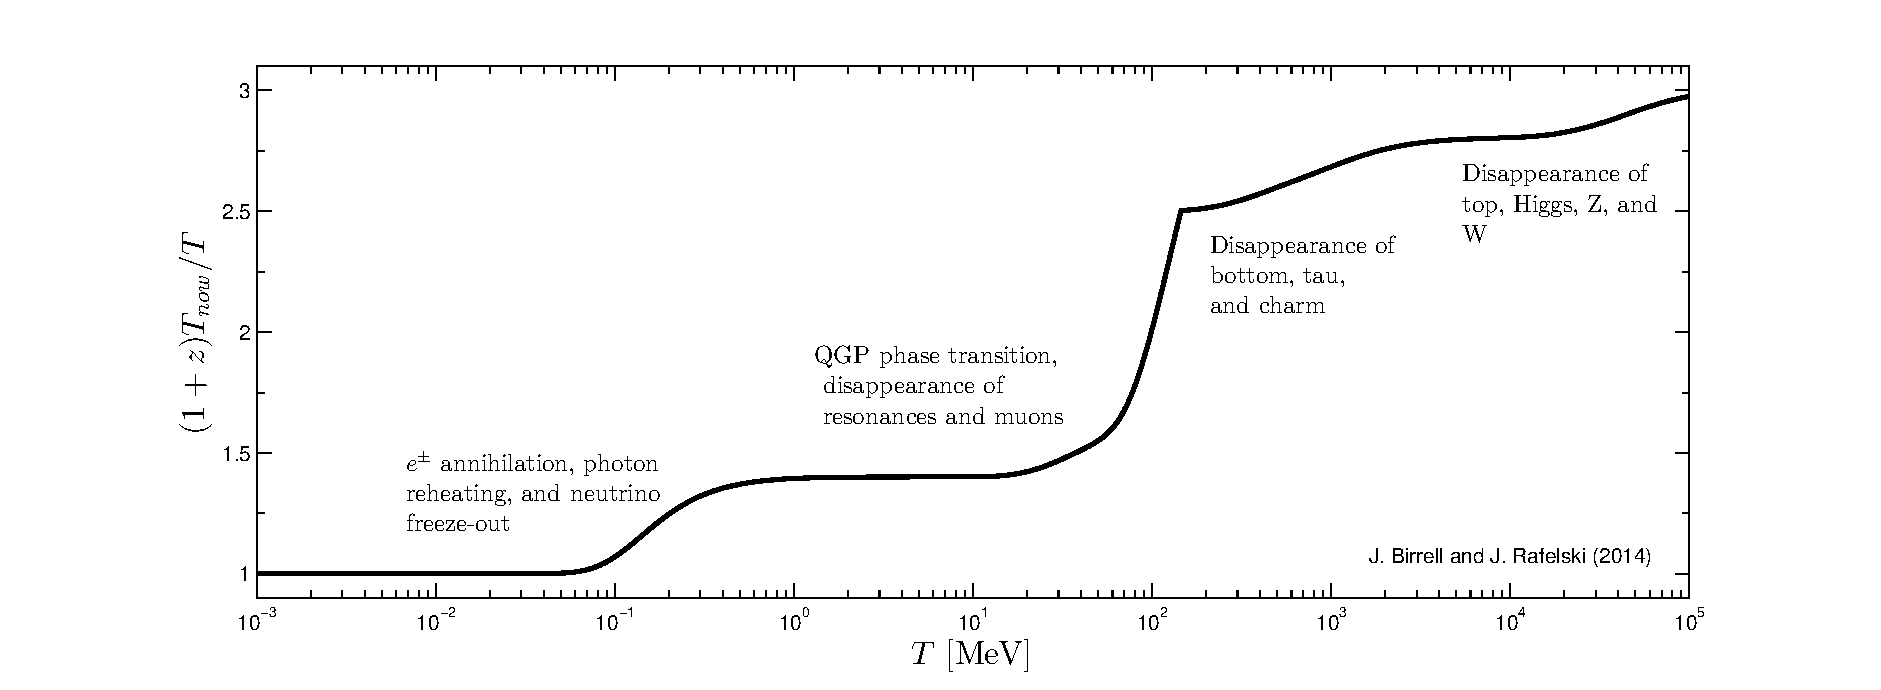
\includegraphics[height=6.6cm]{03-birrell/ErasOfUniverse/z_T_plot.eps}}
\caption{Disappearance of degrees of freedom. The Universe volume inflated approximately by a factor of 27 above the thermal red shift scale as massive particles disappeared successively from the inventory.\label{fig:dof}}
 \end{figure}
%%%%%%%%%%%%%%%%%%%%%%%%%%%%%%%%%%%%%%%



As long as the dynamics are at least approximately entropy conserving, the total drop in $R$ is entirely determined by entropy conservation. Namely, the magnitude of the drop in $R$ figure~\ref{fig:dof} is a measure of the number of degrees of freedom that have disappeared from the Universe. Consider   two times $t_1$ and $t_2$ at which all particle species that have not yet annihilated are effectively massless.  By conservation of comoving entropy and  scaling $T\propto 1/a$ we have
\begin{equation}\label{r_ratio}
1=\frac{a_1^3S_{1}}{a_2^3 S_2}=\frac{a_1^3\sum_ig_i T_{i,1}^3}{a_2^3\sum_j g_j T_{j,2}^3},\qquad \left(\frac{R_1}{R_2}\right)^3=\frac{\sum_ig_i (T_{i,1}/T_{\gamma,1})^3}{\sum_j g_j (T_{j,2}/T_{\gamma,2})^3}
\end{equation}
where the sums are over the total number of degrees of freedom present at the indicated time and the degeneracy factors $g_i$ contain the $7/8$ factor for fermions. In the second form    we divided the numerator and denominator by $a_{0}T_{\gamma,0}$. We distinguish between the temperature of each particle species and our reference temperature, the photon temperature.  This is important since today neutrinos are colder than photons, due to photon reheating from  $e^\pm$ annihilation occurring after neutrinos decoupled (this is only an approximation, a point we will study in detail in subsequent chapters).  By conservation of entropy one obtains the neutrino to photon temperature ratio of
\begin{equation}\label{T_nu_T_gamma}
T_\nu/T_\gamma=({4}/{11})^{1/3}.
\end{equation}
We will call this the reheating ratio in the decoupled limit.  For details on the derivation of this standard result, see for example our paper in appendix \ref{app:model_ind}, where it is obtained as a special case of a more general analysis. 

Using \req{r_ratio}  we  compute the total drop in $R^3$ shown in figure \ref{fig:dof}.  At $T=T_\gamma=\mathcal{O}(100\GeV)$ the number of active degrees of freedom is slightly below $g_{\rm SM}=106.75$ due to the partial disappearance of top quarks, but this approximation will be good enough for our purposes.  At this time, all the species are in thermal equilibrium with photons and so $T_{i,1}/T_{\gamma,1}=1$ for all $i$.  Today we have $2$ photon and $7/8\times 6$ neutrino degrees of freedom and a  neutrino to photon temperature ratio \req{T_nu_T_gamma}.  Therefore we have
\begin{equation}
\left(\frac{R_{100GeV}}{R_{now}}\right)^3= \frac{g_{SM}}{g_{\rm now}}=\frac{106.75}{2+\frac{7}{8}\times 6\times \frac{4}{11}}\approx 27.3
\end{equation}
which is the  fractional change we see in the fermi gas model curve in figure \ref{fig:dof} (as mentioned above, the QCD model is reduced due to interactions). The meaning of this factor is that the Universe approximately inflated by a factor 27 above the thermal red shift scale as massive particles disappeared successively from the inventory. 


\subsection{Composition of the Universe}
From the perspective of reheating, the history of the Universe from the end of $e^\pm$ annihilation until today has been uneventful.  We can shed additional light on this period and others by looking at the composition of the Universe as a function of temperature

%%%%%%%%%%%%%%%%%%%%%%%%%%%%%%%%%%%%
\begin{figure}
\centerline{\hspace*{0.4cm}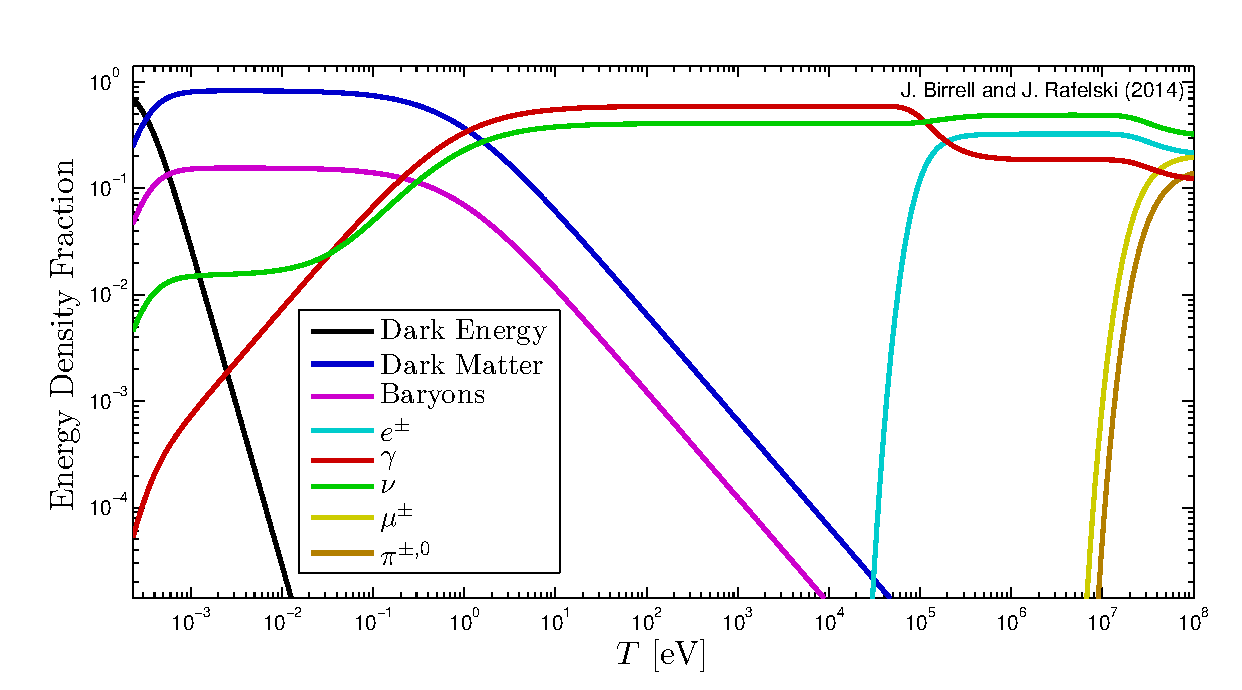
\includegraphics[height=7.6cm]{03-birrell/ErasOfUniverse/energy_densities_total.eps}}\label{fig:energy_frac}
\caption{Current era: $69\%$ dark energy, $26\%$ dark matter, $5\%$ baryons, $<1\%$ photons and neutrinos, $1$ massless and $2\times .1$ eV neutrinos (Neutrino mass choice is just for illustration.  Other values are possible).}
 \end{figure}
%%%%%%%%%%%%%%%%%%%%%%%%%%%%%%%%%%
In figure \ref{fig:energy_frac} we begin on the right at the end of the hadron era with the disappearance of muons and pions.  This constitutes a reheating period, with energy and entropy from these particles being transfered to the remaining $e^\pm$, photon, neutrino plasma.  Continuing to $T=O(1)$ MeV, we come to the annihilation  of $e^\pm$ and the photon reheating period.  Notice that only the photon energy density fraction increases here.  As discussed above, a common simplifying assumption is that neutrinos are already decoupled at this time and hence do not share in the reheating process, leading to a difference in photon and neutrino temperatures \req{T_nu_T_gamma}.

After passing through a long period, from $T=O(1)$ MeV until $T=O(1)$ eV, where the energy density is dominated by photons and free-streaming neutrinos, we then come to the beginning of the matter dominated regime, where the energy density is dominated by dark matter and baryonic matter.  This transition is the result of the redshifting of the photon and neutrino energy, $\rho\propto T^4$, whereas for non-relativistic matter $\rho\propto a^{-3}\propto T^3$.  Note that our inclusion of neutrino mass causes the leveling out of the neutrino energy density fraction during this period, as compared to the continued redshifting of the photon energy.

Finally, as we move towards the present day CMB temperature of $T_{\gamma,0}=0.235$ meV on the left hand side, we have entered the dark energy dominated regime.  For the present day values, we have used the fits from the Planck data \cite{Planck} of  $69\%$ dark energy, $26\%$ dark matter and $5\%$ baryons (and zero spatial curvature).  The photon energy density is fixed by the CMB temperature $T_{\gamma,0}$ and the neutrino energy density is fixed by $T_{\gamma,0}$ along with the photon to neutrino temperature ratio.  Both constitute $<1\%$ of the current energy budget.
In this chapter, we will introduce the fundamental concepts in cosmology for us to explore the properties of the Universe during the `first hour'. I will first present the standard cosmological Friedmann-Lemaitre-Robertson-Walker (FLRW) model, then introduce the general Fermi/Bose distribution with and its application in the early Universe. Finally I present an overview of Universe evolution from $300\,\mathrm{MeV}>T>0.02\,\mathrm{MeV}$.
The Natural unit $c=\hbar=k_{B}=1$ is used throughout the thesis for discussion.
\section{Textbook review: the standard FLRW-Universe model}
%In this section we will focus on the following:
%\begin{itemize}
%    \item The Robertson –Walker Universe
%    \item The Friedmann equation (Hubble %    \item The composition of the universe
%\end{itemize}
The Friedmann-Lemaitre-Robertson-Walker (FLRW) Universe is a theoretical model used widely to describe the cosmological evolution of the Universe. It is based on the cosmological principles which assumes homogeneity and isotropy of the Universe on large scales. In general, the FLRW metric can be written as
\begin{align}\label{metric}
ds^2=c^2dt^2-a^2(t)\left[ \frac{dr^2}{1-kr^2}+r^2(d\theta^2+\sin^2\theta\,d\phi^2)\right].
\end{align}
The metric is characterized by the scale factor $a(t)$ which measures the size of the Universe as a function of time $t$. The geometric parameter $k$ identifies the Gaussian geometry of the spatial hyper-surfaces defined by co-moving observers. The metrics are qualitatively different depending on the value of $k$. We have $k=1$ which correspond to the closed Universe,  $k=0$ correspond to flat Universe, and $k=-1$ for open geometries of the Universe. Current observation of cosmic microwave background (CMB) anisotropy preferred value $k=0$~[\cite{Planck:2013pxb,Planck:2015fie,Planck:2018vyg}].
\include{03-birrell/birrell}
\include{04-grayson/grayson}
%%%%%%%%%%%%%%%%%%%%%%%%%%%%%%%%%%%%%%%
%\chapter{Matter-antimatter origin of cosmic magnetism}
%\label{chap:cosmo}
%%%%%%%%%%%%%%%%%%%%%%%%%%%%%%%%%%%%%%%
\noindent We investigate the hypothesis that the observed intergalactic magnetic fields (IGMF) are primordial in nature, predating the recombination epoch. Specifically, we explore the role of the extremely large electron-positron $(e^{+}e^{-})$ pair abundance in the temperature range of $2000\keV>T>20\keV$ which only disappeared after Big Bang nucleosynthesis (BBN). We review the status of cosmic magnetism in \rsec{sec:universe} which motivates our study. \rsec{sec:abundance} discusses the extreme electron-positron abundance during this epoch. The statistical and thermodynamic theory of the electron-positron gas is described in \rsec{sec:theory}. \rsec{sec:magnetization} describes the relativistic paramagnetism of the electron-positron gas. We propose in \rsec{sec:ferro} a model of self-magnetization caused by spin polarization within the individual species in the gas.

This chapter serves primarily as a review of our work in~\cite{Steinmetz:2023nsc,Steinmetz:2023ucp} and portions of~\cite{Rafelski:2023emw} where we propose that the early universe electron-positron plasma was a highly magnetized environment. We will use natural units $(c=\hbar=k_{B}=1)$ unless otherwise noted.

%%%%%%%%%%%%%%%%%%%%%%%%%%%%%%%%%%%%%%%
\section{Short survey of magnetism in the universe}
\label{sec:universe}
%%%%%%%%%%%%%%%%%%%%%%%%%%%%%%%%%%%%%%%
\noindent Macroscopic domains of magnetic fields have been found in all astrophysical environments from compact objects (stars, planets, etc.); interstellar and intergalactic space; and surprisingly in deep extra-galactic void spaces. Considering the ubiquity of magnetic fields in the universe~\cite{Giovannini:2017rbc,Giovannini:2003yn,Kronberg:1993vk}, we search for a common primordial mechanism initiate the diversity of magnetism observed today. In this chapter, IGMF will refer to experimentally observed intergalactic fields of any origin while primordial magnetic fields (PMF) refers to fields generated via early universe processes possibly as far back as inflation. The conventional elaboration of the origins for cosmic PMFs are detailed in~\cite{Gaensler:2004gk,Durrer:2013pga,AlvesBatista:2021sln}.

IGMF are notably difficult to measure and difficult to explain. The bounds for IGMF at a length scale of $1{\rm\ Mpc}$ are today~\cite{Neronov:2010gir,Taylor:2011bn,Pshirkov:2015tua,Jedamzik:2018itu,Vernstrom:2021hru}
\begin{gather}
 \label{igmf}
 10^{-8}{\rm\ G}>B_\mathrm{IGMF}>10^{-16}{\rm\ G}\,.
\end{gather}
We note that generating PMFs with such large coherent length scales is nontrivial~\cite{Giovannini:2022rrl} though currently the length scale for PMFs are not well constrained~\cite{AlvesBatista:2021sln}. Faraday rotation from distant radio active galaxy nuclei (AGN)~\cite{Pomakov:2022cem} suggest that neither dynamo nor astrophysical processes would sufficiently account for the presence of magnetic fields in the universe today if the IGMF strength was around the upper bound of $B_\mathrm{IGMF}\simeq30-60{\rm\ nG}$ as found in Ref.~\cite{Vernstrom:2021hru}. Such strong magnetic fields would then require that at least some portion of the IGMF arise from primordial sources that predate the formation of stars.

Magnetized baryon inhomogeneities which in turn would produce anisotropies in the cosmic microwave background (CMB)~\cite{Jedamzik:2013gua,Abdalla:2022yfr}. \cite{Jedamzik:2020krr} propose further that the presence of a magnetic field of $B_\mathrm{PMF}\simeq0.1{\rm\ nG}$ could be sufficient to explain the Hubble tension.

%%%%%%%%%%%%%%%%%%%%%%%%%%%%%%%%%%%%%%%
\begin{figure}[ht]
    \centering
    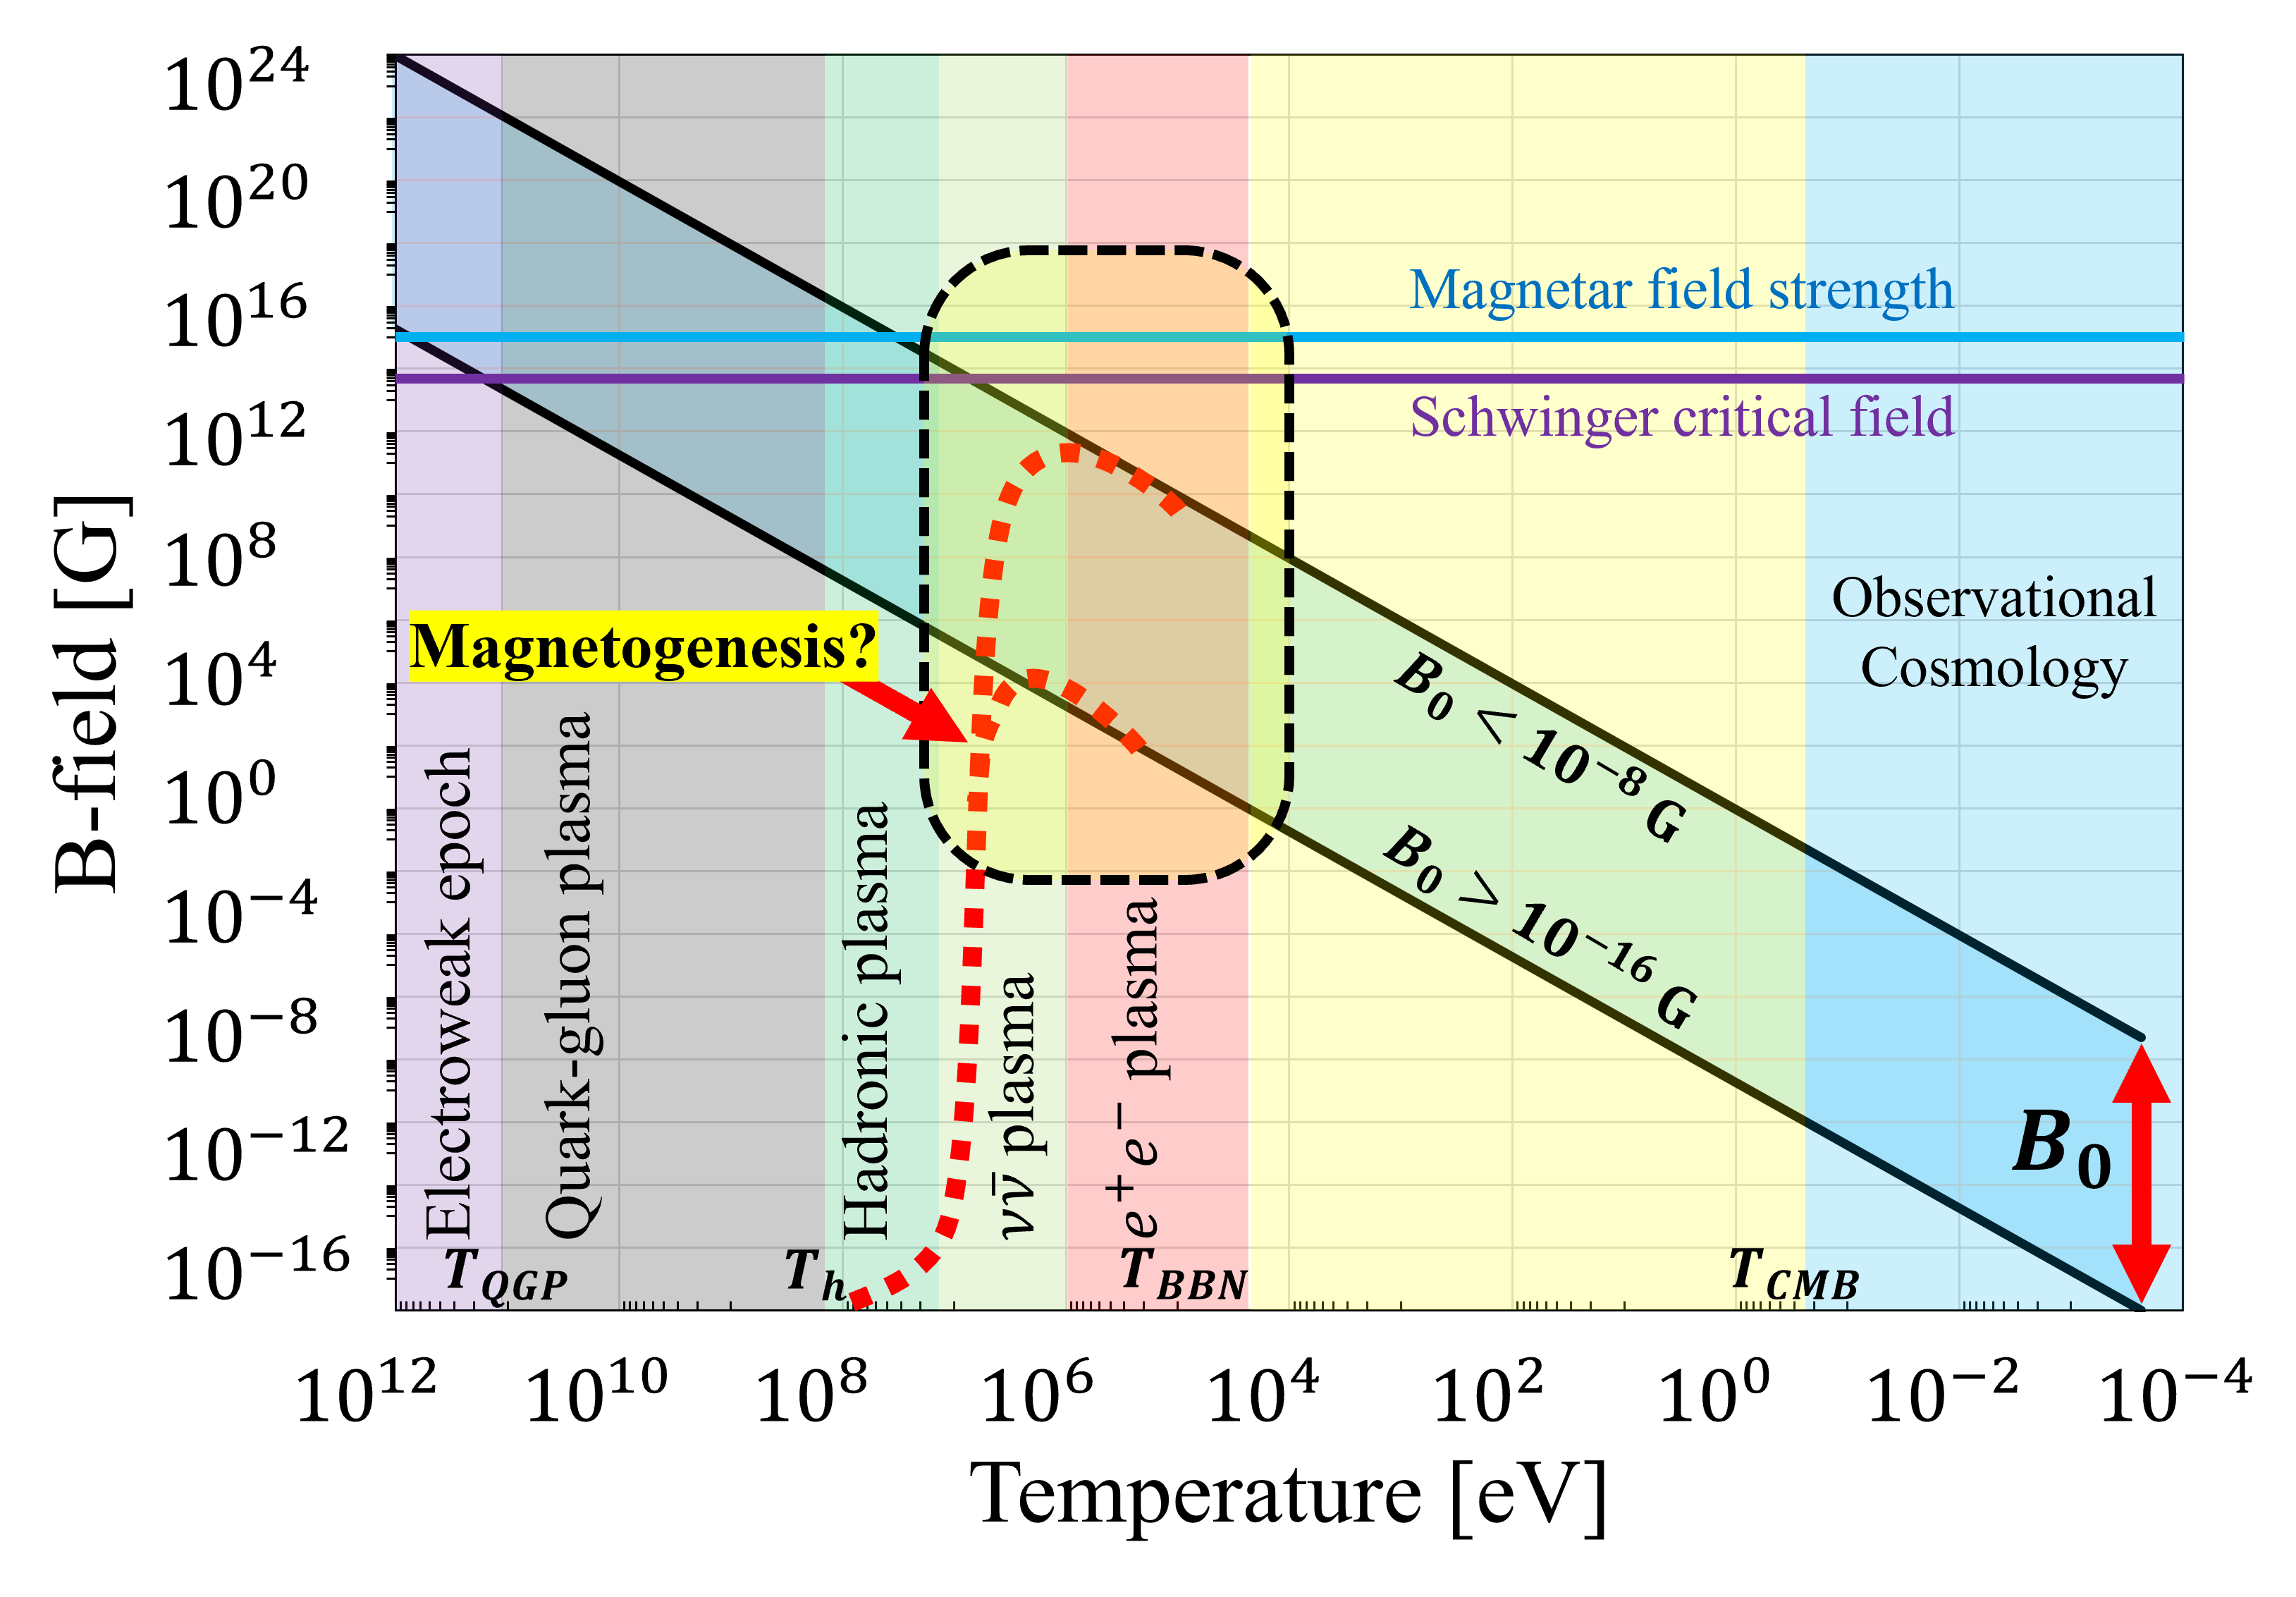
\includegraphics[width=0.95\textwidth]{plots/chap04cosmo/pmf.png}
    \caption{Qualitative plot of the primordial magnetic field strength over cosmic time. All figures are printed in temporal sequence in the expanding universe beginning with high temperatures (and early times) on the left and lower temperatures (and later times) on the right.}
    \label{fig:pmf}
\end{figure}
%%%%%%%%%%%%%%%%%%%%%%%%%%%%%%%%%%%%%%%

Our motivating hypothesis is outlined qualitatively in \rf{fig:pmf} where PMF evolution is plotted over the temperature history of the universe. The descending blue band indicates the range of possible PMF strengths. The different epochs of the universe according to $\Lambda\mathrm{CDM}$ are delineated by temperature. The horizontal lines mark two important scales: (a) the Schwinger critical field strength given by
\begin{align}
    \label{crit:1}
    B_\mathrm{C} = \frac{m_{e}^{2}}{e}\simeq4.41\times10^{13}\,\mathrm{G}\,.
\end{align}
where electrodynamics is expected to display nonlinear characteristics and (b) the upper field strength seen in magnetars of $\sim10^{15}\,\mathrm{G}$. A schematic of magnetogenesis is drawn with the dashed red lines indicating spontaneous formation of the PMF within the early universe plasma itself. The $e^{+}e^{-}$ era is notably the final epoch where antimatter exists in large quantities in the cosmos~\cite{Rafelski:2023emw}.

%%%%%%%%%%%%%%%%%%%%%%%%%%%%%%%%%%%%%%%
\section{Electron-positron abundance}
\label{sec:abundance}
%%%%%%%%%%%%%%%%%%%%%%%%%%%%%%%%%%%%%%%
\noindent As the universe cooled below temperature $T\!=\!m_{e}$ (the electron mass), the thermal electron and positron comoving density depleted by over eight orders of magnitude. At $T_\mathrm{split}=20.3\keV$, the charged lepton asymmetry (mirrored by baryon asymmetry and enforced by charge neutrality) became evident as the surviving excess electrons persisted while positrons vanished entirely from the particle inventory of the universe due to annihilation.

%%%%%%%%%%%%%%%%%%%%%%%%%%%%%%%%%%%%%%%
\begin{figure}[ht]
 \centering
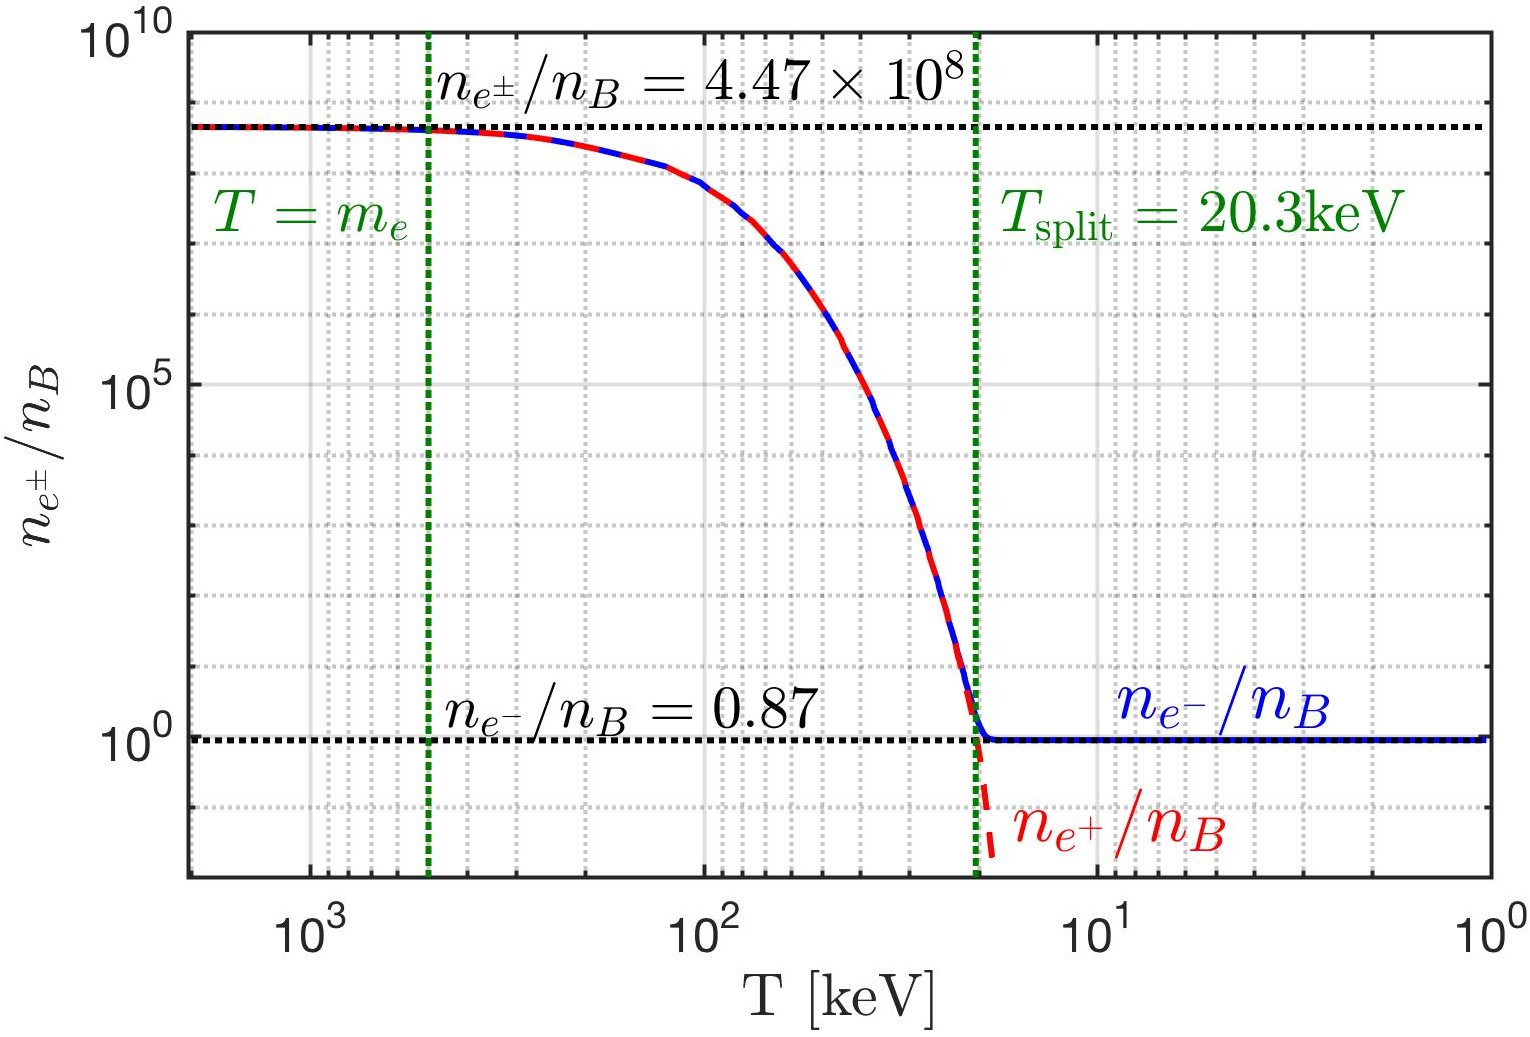
\includegraphics[width=0.95\textwidth]{plots/chap04cosmo/EEPlasmaDensityRatio_new01.jpg}
 \caption{Number density of electron $e^{-}$ and positron $e^{+}$ to baryon ratio $n_{e^{\pm}}/n_{B}$ as a function of photon temperature in the universe. See text for further details. In this work we measure temperature in units of energy (keV) thus we set the Boltzmann constant to $k_{B}=1$. Figure courtesy of Cheng Tao Yang.}
 \label{fig:densityratio} 
\end{figure}
%%%%%%%%%%%%%%%%%%%%%%%%%%%%%%%%%%%%%%%

The electron-to-baryon density ratio $n_{e^{-}}/n_{B}$ is shown in \rf{fig:densityratio} as the solid blue line while the positron-to-baryon ratio $n_{e^{+}}/n_{B}$ is represented by the dashed red line. These two lines overlap until the temperature drops below $T_\mathrm{split}=20.3\keV$ as positrons vanish from the universe marking the end of the $e^{+}e^{-}$ plasma and the dominance of the electron-proton $(e^{-}p)$ plasma. The two vertical dashed green lines denote temperatures $T\!=\!m_{e}\simeq511\keV$ and $T_\mathrm{split}=20.3\keV$. These results were obtained using charge neutrality and the baryon-to-photon content (entropy) of the universe; see details in~\cite{Rafelski:2023emw}. The two horizontal black dashed lines denote the relativistic $T\gg m_e$ abundance of $n_{e^{\pm}}/n_{B}=4.47\times10^{8}$ and post-annihilation abundance of $n_{e^{-}}/n_{B}=0.87$. Above temperature $T\simeq85\keV$, the $e^{+}e^{-}$ primordial plasma density exceeded that of the Sun's core density $n_{e}\simeq6\times10^{26}{\rm\ cm}^{-3}$~\cite{Bahcall:2000nu}. 

Conversion of the dense $e^{+}e^{-}$ pair plasma into photons reheated the photon background~\cite{Birrell:2014uka} separating the photon and neutrino temperatures. The $e^{+}e^{-}$ annihilation and photon reheating period lasted no longer than an afternoon lunch break. Because of charge neutrality, the post-annihilation comoving ratio $n_{e^{-}}/n_{B}=0.87$~\cite{Rafelski:2023emw} is slightly offset from unity in~\rf{fig:densityratio} by the presence of bound neutrons in $\alpha$ particles and other neutron containing light elements produced during BBN epoch.

The abundance of baryons is itself fixed by the known abundance relative to photons~\cite{ParticleDataGroup:2022pth} and we employed the contemporary recommended value $n_B/n_\gamma=6.09\times 10^{-10}$. The resulting chemical potential needs to be evaluated carefully to obtain the behavior near to $T_\mathrm{split}=20.3\keV$ where the relatively small value of chemical potential $\mu$ rises rapidly so that positrons vanish from the particle inventory of the universe while nearly one electron per baryon remains. The detailed solution of this problem is found in \cite{Fromerth:2012fe,Rafelski:2023emw} leading to the results shown in \rf{fig:densityratio}.

%%%%%%%%%%%%%%%%%%%%%%%%%%%%%%%%%%%%%%%
\section{Theory of thermal matter-antimatter plasmas}
\label{sec:theory}
%%%%%%%%%%%%%%%%%%%%%%%%%%%%%%%%%%%%%%%
\noindent To evaluate magnetic properties of the thermal $e^{+}e^{-}$ pair plasma we take inspiration from Ch. 9 of Melrose's treatise on magnetized plasmas~\cite{melrose2008quantum}. We focus on the bulk properties of thermalized plasmas in (near) equilibrium.

We consider a homogeneous magnetic field domain defined along the $z$-axis as
\begin{gather}
    \label{homoB:1}
    \bb{B}=(0,\,0,\,B)\,,
\end{gather}
with magnetic field magnitude $|\bb{B}|=B$. Following \rchap{chap:moment}, we reprint the microscopic energy (\req{lan24b} in different notation) of the charged relativistic fermion within a homogeneous magnetic field given by
\begin{align}
 \label{cosmokgp}
 E^{n}_{\sigma,s}(p_{z},{B})=\sqrt{m_{e}^{2}+p_{z}^{2}+e{B}\left(2n+1+\frac{g}{2}\sigma s\right)}\,,
\end{align}
where $n\in0,1,2,\ldots$ is the Landau orbital quantum number, $p_{z}$ is the momentum parallel to the field axis and the electric charge is $e\equiv q_{e^{+}}=-q_{e^{-}}$. The index $\sigma$ in \req{cosmokgp} differentiates electron $(e^{-};\ \sigma=+1)$ and positron $(e^{+};\ \sigma=-1)$ states. The index $s$ refers to the spin along the field axis: parallel $(\uparrow;\ s=+1)$ or anti-parallel $(\downarrow;\ s=-1)$ for both particle and antiparticle species.

%%%%%%%%%%%%%%%%%%%%%%%%%%%%%%%%%%%%%%%
\begin{figure}[ht]
 \centering
 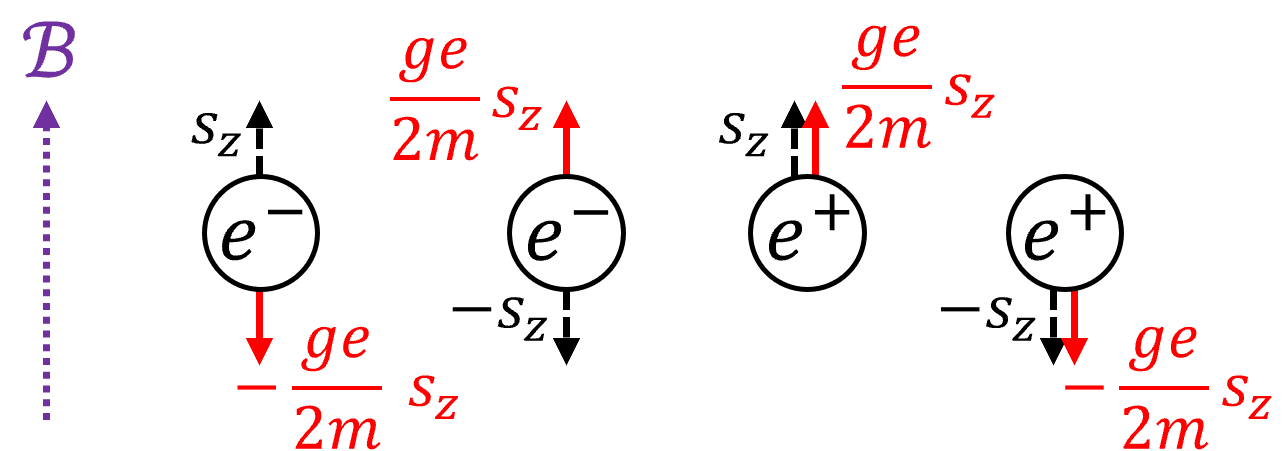
\includegraphics[width=0.95\linewidth]{plots/chap04cosmo/schematic.png}\Bstrut\\
 \begin{tabular}{ r|c|c| }
 \multicolumn{1}{r}{}
 & \multicolumn{1}{c}{aligned: $s=+1$}
 & \multicolumn{1}{c}{anti-aligned: $s=-1$} \\
 \cline{2-3}
 electron: $\sigma=+1$ & $U_{\rm Mag}>0$ & $U_{\rm Mag}<0$ \TBstrut\\
 \cline{2-3}
 positron: $\sigma=-1$ & $U_{\rm Mag}<0$ & $U_{\rm Mag}>0$ \TBstrut\\
 \cline{2-3}
 \end{tabular}\\
 \caption{Organizational schematic of matter-antimatter $(\sigma)$ and polarization $(s)$ states with respect to the sign of the non-relativistic magnetic dipole energy $U_{\rm Mag}$ obtainable from~\req{cosmokgp}.}
 \label{fig:schematic}
\end{figure}
%%%%%%%%%%%%%%%%%%%%%%%%%%%%%%%%%%%%%%%

The reason \req{cosmokgp} distinguishes between electrons and positrons is to ensure the correct non-relativistic limit for the magnetic dipole energy is reached. Following the conventions found in \cite{Tiesinga:2021myr}, we set the gyro-magnetic factor $g\equiv g_{e^{+}}=-g_{e^{-}}>0$ such that electrons and positrons have opposite $g$-factors and opposite magnetic moments relative to their spin; see \rf{fig:schematic}.

We recall the conventions established in \rsec{sec:flrw}. Conservation of magnetic flux requires that the magnetic field through a comoving surface $L_{0}^{2}$ remain unchanged. The magnetic field strength under expansion~\cite{Durrer:2013pga} starting at some initial time $t_{0}$ is then given by
\begin{gather}
 \label{bscale}
 B(t)=B_{0}\frac{a^{2}_{0}}{a^{2}(t)}\rightarrow B(z)=B_{0}\left(1+z\right)^{2}\,,
\end{gather}
where $B_{0}$ is the comoving value obtained from the contemporary value of the magnetic field today. Magnetic fields in the cosmos generated through mechanisms such as dynamo or astrophysical sources do not follow this scaling~\cite{Pomakov:2022cem}. It is only in deep intergalactic space where matter density is low are magnetic fields preserved (and thus uncontaminated) over cosmic time.

From \req{tscale} and \req{bscale} there emerges a natural ratio of interest which is conserved over cosmic expansion 
\begin{gather}
 \label{tbscale}
 \boxed{b\equiv\frac{e{B}(t)}{T^{2}(t)}=\frac{e{B}_{0}}{T_{0}^{2}}\equiv b_0={\rm\ const.}}\\
 10^{-3}>b_{0}>10^{-11}\,,
\end{gather}
given in natural units ($c=\hbar=k_{B}=1$). We computed the bounds for this cosmic magnetic scale ratio by using the present day IGMF observations given by \req{igmf} and the present CMB temperature $T_{0}=2.7{\rm\ K}\simeq2.3\times10^{-4}\eV$~\cite{Planck:2018vyg}.

%%%%%%%%%%%%%%%%%%%%%%%%%%%%%%%%%%%%%%%
\subsection{Eigenstatess of magnetic moment in cosmology}
\label{sec:protection}
%%%%%%%%%%%%%%%%%%%%%%%%%%%%%%%%%%%%%%%

As statistical properties depend on the characteristic Boltzmann factor $E/T$, another interpretation of \req{tbscale} in the context of energy eigenvalues (such as those given in \req{cosmokgp}) is the preservation of magnetic moment energy relative to momentum under adiabatic cosmic expansion. The Boltzmann statistical factor is given by
\begin{alignat}{1}
    \label{Boltz} x\equiv\frac{E}{T}\,.
\end{alignat}
We can explore this relationship for the magnetized system explicitly by writing out \req{Boltz} using the KGP energy eigenvalues written in \req{cosmokgp} as
\begin{alignat}{1}
    \label{XExplicit} x_{\sigma,s}^{n} = \frac{E_{\sigma,s}^{n}}{T} = \sqrt{\frac{m_{e}^{2}}{T^{2}}+\frac{p_{z}^{2}}{T^{2}}+\frac{eB}{T^{2}}\left(2n+1+\frac{g}{2}\sigma s\right)}\,.
\end{alignat}

Introducing the expansion scale factor $a(t)$ via \req{tscale}, \req{bscale} and \req{tbscale}. The Boltzmann factor can then be written as
\begin{alignat}{1}
    \label{xscale:1} x_{\sigma,s}^{n}(a(t)) = \sqrt{\frac{m_{e}^{2}}{T^{2}(t_{0})}\frac{a(t)^{2}}{a_{0}^{2}}+\frac{p_{z,0}^{2}}{T_{0}^{2}}+\frac{eB_{0}}{T_{0}^{2}}\left(2n+1+\frac{g}{2}\sigma s\right)}\,.
\end{alignat}
This reveals that only the mass contribution is dynamic over cosmological time. The constant of motion $b_{0}$ defined in \req{tbscale} is seen as the coefficient to the Landau and spin portion of the energy. For any given eigenstate, the mass term drives the state into the non-relativistic limit while the momenta and magnetic contributions are frozen by initial conditions. 

In comparison, the Boltzmann factor for the DP energy eigenvalues are given by
\begin{alignat}{1}
    \label{xscaledp:1} x_{\sigma,s}^{n}\vert_\mathrm{DP} = \sqrt{\left(\sqrt{\frac{m_{e}^{2}}{T^{2}}+\frac{eB}{T^{2}}\left(2n+1+\sigma s\right)}+\frac{eB}{2m_{e}T}\left(\frac{g}{2}-1\right)\sigma s\right)^{2}+\frac{p_{z}^{2}}{T^{2}}}\,,
\end{alignat}
which scales during FLRW expansion as
\begin{multline}
    \label{xscaledp:2} x_{\sigma,s}^{n}(a(t))\vert_\mathrm{DP} =\\ \sqrt{\left(\sqrt{\frac{m_{e}^{2}}{T_{0}^{2}}\frac{a(t)^{2}}{a_{0}^{2}}+\frac{eB_{0}}{T_{0}^{2}}\left(2n+1+\sigma s\right)}+\frac{eB_{0}}{2m_{e}T_{0}}\frac{a_{0}}{a(t)}\left(\frac{g}{2}-1\right)\sigma s\right)^{2}+\frac{p_{z,0}^{2}}{T_{0}^{2}}}\,.
\end{multline}
While the above expression is rather complicated, we note that the KGP~\req{xscale:1} and DP~\req{xscaledp:1} Boltzmann factors both reduce to the Sch{\"o}dinger-Pauli limit as $a(t)\rightarrow\infty$ thereby demonstrating that the total magnetic moment is protected under the adiabatic expansion of the universe.

As noted in in \rsec{sec:ikgp} and \rsec{sec:emmass}, higher order non-minimal magnetic contributions can be introduced to the Boltzmann factor such as $\sim(e/m)^{2}B^{2}/T^{2}$. The reasoning above suggests that these terms are suppressed over cosmological time driving the system into minimal electromagnetic coupling with the exception of the anomalous magnetic moment. It is interesting to note that cosmological expansion then serves to `smooth out' the characteristics of more complex electrodynamics erasing them from a statistical perspective in favor of minimal-like dynamics.

%%%%%%%%%%%%%%%%%%%%%%%%%%%%%%%%%%%%%%%
\subsection{Magnetized fermion partition function}
\label{sec:partition}
%%%%%%%%%%%%%%%%%%%%%%%%%%%%%%%%%%%%%%%
\noindent To obtain a quantitative description of the above evolution, we study the bulk properties of the relativistic charged/magnetic gasses in a nearly homogeneous and isotropic primordial universe via the thermal Fermi-Dirac or Bose distributions.

The grand partition function for the relativistic Fermi-Dirac ensemble is given by the standard definition
\begin{alignat}{1}
    \label{part:1} \ln\mathcal{Z}_\mathrm{total}=\sum_{\alpha}\ln\left(1+\Upsilon_{\alpha_{1}\ldots\alpha_{m}}\exp\left(-\frac{E_{\alpha}}{T}\right)\right)\,,\qquad\Upsilon_{\alpha_{1}\ldots\alpha_{m}}=\lambda_{\alpha_{1}}\lambda_{\alpha_{2}}\ldots\lambda_{\alpha_{m}}
\end{alignat}
where we are summing over the set all relevant quantum numbers $\alpha=(\alpha_{1},\alpha_{2},\ldots,\alpha_{m})$. We note here the generalized the fugacity $\Upsilon_{\alpha_{1}\ldots\alpha_{m}}$ allowing for any possible deformation caused by pressures effecting the distribution of any quantum numbers.

In the case of the Landau problem, there is an additional summation over $\widetilde{G}$ which represents the occupancy of Landau states~\cite{greiner2012thermodynamics} which are matched to the available phase space within $\Delta p_{x}\Delta p_{y}$. If we consider the orbital Landau quantum number $n$ to represent the transverse momentum $p_{T}^{2}=p_{x}^{2}+p_{y}^{2}$ of the system, then the relationship that defines $\widetilde{G}$ is given by
\begin{alignat}{1}
    \label{phase:1} \frac{L^{2}}{(2\pi)^{2}}\Delta p_{x}\Delta p_{y}=\frac{eBL^{2}}{2\pi}\Delta n\,,\qquad\widetilde{G}=\frac{eBL^{2}}{2\pi}\,.
\end{alignat}
The summation over the continuous $p_{z}$ is replaced with an integration and the double summation over $p_{x}$ and $p_{y}$ is replaced by a single sum over Landau orbits
\begin{alignat}{1}
    \label{phase:2}
    \sum_{p_{z}}\rightarrow\frac{L}{2\pi}\int^{+\infty}_{-\infty}dp_{z}\,,\qquad\sum_{p_{x}}\sum_{p_{y}}\rightarrow\frac{eBL^{2}}{2\pi}\sum_{n}\,,
\end{alignat}
where $L$ defines the boundary length of our considered volume $V=L^{3}$.

The partition function of the $e^{+}e^{-}$ plasma can be understood as the sum of four gaseous species
\begin{align}
    \label{partition:0}    
    \ln\mathcal{Z}_{e^{+}e^{-}}=\ln\mathcal{Z}_{e^{+}}^{\uparrow}+\ln\mathcal{Z}_{e^{+}}^{\downarrow}+\ln\mathcal{Z}_{e^{-}}^{\uparrow}+\ln\mathcal{Z}_{e^{-}}^{\downarrow}\,,
\end{align}
of electrons and positrons of both polarizations $(\uparrow\downarrow)$. The change in phase space written in \req{phase:2} modify the magnetized $e^{+}e^{-}$ plasma partition function from \req{part:1} into
\begin{gather}
     \label{partition:1}
     \ln\mathcal{Z}_{e^{+}e^{-}}=\frac{e{B}V}{(2\pi)^{2}}\sum_{\sigma}^{\pm1}\sum_{s}^{\pm1}\sum_{n=0}^{\infty}\int_{-\infty}^{\infty}\mathrm{d}p_{z}\left[\ln\left(1+\lambda_{\sigma}\xi_{\sigma,s}\exp\left(-\frac{E_{\sigma,s}^{n}}{T}\right)\right)\right]\,\\
    \label{partition:2}    
    \Upsilon_{\sigma,s} =\lambda_{\sigma}\xi_{\sigma,s} = \exp{\frac{\mu_{\sigma}+\eta_{\sigma,s}}{T}}\,,
\end{gather}
where the energy eigenvalues $E_{\sigma,s}^{n}$ are given in \req{cosmokgp}. The index $\sigma$ in \req{partition:1} is a sum over electron and positron states while $s$ is a sum over polarizations. The index $s$ refers to the spin along the field axis: parallel $(\uparrow;\ s=+1)$ or anti-parallel $(\downarrow;\ s=-1)$ for both particle and antiparticle species.

We are explicitly interested in small asymmetries such as baryon excess over antibaryons, or one polarization over another. These are described by \req{partition:2} as the following two fugacities:
\begin{itemize}[nosep]
 \item[(a)] Chemical fugacity $\lambda_{\sigma}$
 \item[(b)] Polarization fugacity $\xi_{\sigma,s}$
\end{itemize}
For matter $(e^{-};\ \sigma=+1)$ and antimatter $(e^{+};\ \sigma=-1)$ particles, a nonzero relativistic chemical potential $\mu_{\sigma}=\sigma\mu$ is caused by an imbalance of matter and antimatter. While the primordial electron-positron plasma era was overall charge neutral, there was a small asymmetry in the charged leptons (namely electrons) from baryon asymmetry~\cite{Fromerth:2012fe,Canetti:2012zc} in the universe. Reactions such as $e^{+}e^{-}\leftrightarrow\gamma\gamma$ constrains the chemical potential of electrons and positrons~\cite{Elze:1980er} as 
\begin{align}
 \label{cpotential}
 \mu\equiv\mu_{e^{-}}=-\mu_{e^{+}}\,,\qquad
 \lambda\equiv\lambda_{e^{-}}=\lambda_{e^{+}}^{-1}=\exp\frac{\mu}{T}\,,
\end{align}
where $\lambda$ is the chemical fugacity of the system.

We can then parameterize the chemical potential of the $e^{+}e^{-}$ plasma as a function of temperature $\mu\rightarrow\mu(T)$ via the charge neutrality of the universe which implies
\begin{align}
 \label{chargeneutrality}
 n_{p}=n_{e^{-}}-n_{e^{+}}=\frac{1}{V}\lambda\frac{\partial}{\partial\lambda}\ln\mathcal{Z}_{e^{+}e^{-}}\,.
\end{align}
In \req{chargeneutrality}, $n_{p}$ is the observed total number density of protons in all baryon species. The chemical potential defined in \req{cpotential} is obtained from the requirement that the positive charge of baryons (protons, $\alpha$ particles, light nuclei produced after BBN) is exactly and locally compensated by a tiny net excess of electrons over positrons.

We then introduce a novel polarization fugacity $\xi_{\sigma,s}$ and polarization potential $\eta_{\sigma,s}=\sigma s\eta$. We propose the polarization potential follows analogous expressions as seen in \req{cpotential} obeying
\begin{align}
 \label{spotential}
 \eta\equiv\eta_{+,+}=\eta_{-,-}\,,\quad\eta=-\eta_{\pm,\mp}\,,\quad\xi_{\sigma,s}\equiv\exp{\frac{\eta_{\sigma,s}}{T}}\,.
\end{align}
An imbalance in polarization within a region of volume $V$ results in a nonzero polarization potential $\eta\neq0$. Conveniently since antiparticles have opposite signs of charge and magnetic moment, the same magnetic moment is associated with opposite spin orientations. A completely particle-antiparticle symmetric magnetized plasma will have therefore zero total angular momentum.

%%%%%%%%%%%%%%%%%%%%%%%%%%%%%%%%%%%%%%%
\subsubsection{Euler-Maclaurin integration}
\label{sec:eulermac}
%%%%%%%%%%%%%%%%%%%%%%%%%%%%%%%%%%%%%%%
\noindent Before we proceed with the Boltzmann distribution approximation which makes up the bulk of our analysis, we will comment on the full Fermi-Dirac distribution analysis. The Euler-Maclaurin formula~\cite{abramowitz1988handbook} is used to convert the summation over Landau levels $n$ into an integration given by
\begin{multline}
    \label{eulermaclaurin}\sum^{b}_{n=a}f(n)-\int^{b}_{a}f(x)dx = \frac{1}{2}\left(f(b)+f(a)\right)\\
    +\sum_{i=1}^{j}\frac{b_{2i}}{(2i)!}\left(f^{(2i-1)}(b)-f^{(2i-1)}(a)\right)+R(j)\,,
\end{multline}
where $b_{2i}$ are the Bernoulli numbers and $R(j)$ is the error remainder defined by integrals over Bernoulli polynomials. The integer $j$ is chosen for the level of approximation that is desired. Euler-Maclaurin integration is rarely convergent, and in this case serves only as an approximation within the domain where the error remainder is small and bounded; see~\cite{greiner2012thermodynamics} for the non-relativistic case. In this analysis, we keep the zeroth and first order terms in the Euler-Maclaurin formula. We note that regularization of the excess terms in \req{eulermaclaurin} is done in the context of strong field QED~\cite{greiner2008quantum} though that is outside our scope.

Using \req{eulermaclaurin} allows us to convert the sum over $n$ quantum numbers in \req{partition:1} into an integral. Defining
\begin{alignat}{1}
    \label{Func} f_{\sigma,s}^{n}=\ln\left(1+\Upsilon_{\sigma,s}\exp\left(-\frac{E_{\sigma,s}^{n}}{T}\right)\right)\,,
\end{alignat}
\req{partition:1} for $j=1$ becomes
\begin{multline}
    \label{PartFuncTwo} \ln\mathcal{Z}_{e^{+}e^{-}} = \frac{e{B}V}{(2\pi)^{2}}\sum_{\sigma,s}^{\pm1}\int_{-\infty}^{+\infty}dp_{z}\\
    \left(\int_{0}^{+\infty}dn f_{\sigma,s}^{n} + \frac{1}{2}f_{\sigma,s}^{0} + \frac{1}{12}\frac{\partial f_{\sigma,s}^{n}}{\partial n}\bigg\rvert_{n=0} + R(1)\right)
\end{multline}
It will be useful to rearrange \req{cosmokgp} by pulling the spin dependency and the ground state Landau orbital into the mass writing
\begin{gather}
 \label{effmass:1}
 E^{n}_{\sigma,s}={\tilde m}_{\sigma,s}\sqrt{1+\frac{p_{z}^{2}}{{\tilde m}_{\sigma,s}^{2}}+\frac{2e{B}n}{{\tilde m}_{\sigma,s}^{2}}}\,,\\
 \label{effmass:2}
 \varepsilon_{\sigma,s}^{n}(p_{z},{B})=\frac{E_{\sigma,s}^{n}}{{\tilde m}_{\sigma,s}}\,,\qquad{\tilde m}_{\sigma,s}^{2}=m_{e}^{2}+e{B}\left(1+\frac{g}{2}\sigma s\right)\,,
\end{gather}
where we introduced the dimensionless energy $\varepsilon^{n}_{\sigma,s}$ and effective polarized mass ${\tilde m}_{\sigma,s}$ which is distinct for each spin alignment and is a function of magnetic field strength ${B}$. The effective polarized mass ${\tilde m}_{\sigma,s}$ allows us to describe the $e^{+}e^{-}$ plasma with the spin effects almost wholly separated from the Landau characteristics of the gas when considering the plasma's thermodynamic properties.

With the energies written in this fashion, we recognize the first term in \req{PartFuncTwo} as mathematically equivalent to the free particle fermion partition function with a re-scaled mass $m_{\sigma,s}$. The phase-space relationship between transverse momentum and Landau orbits in \req{phase:1} and \req{phase:2} can be succinctly described by
\begin{gather}
    p_{T}^{2} \sim 2eBn\,,\qquad2p_{T}dp_{T} \sim 2eBdn\,,\qquad d\bb{p}^{3}=2\pi p_{T}dp_{T}dp_{z}\\
    \frac{eBV}{(2\pi)^{2}}\int_{-\infty}^{+\infty}dp_{z}\int_{0}^{+\infty}dn \rightarrow \frac{V}{(2\pi)^{3}}\int d\bb{p}^{3}
\end{gather}
which recasts the first term in \req{PartFuncTwo} as
\begin{align}
    \label{FreePart}
    \ln\mathcal{Z}_{e^{+}e^{-}} = \frac{V}{(2\pi)^{3}}\sum_{\sigma,s}^{\pm1}\int d\bb{p}^{3}\ln\left(1+\Upsilon_{\sigma,s}\exp{\left(-\frac{m_{\sigma,s}\sqrt{1+p^{2}/m_{\sigma,s}^{2}}}{T}\right)}\right)+\ldots
\end{align}
As we will see in the proceeding section, this separation of the `free-like' partition function can be reproduced in the Boltzmann distribution limit as well. This marks the end of the analytic analysis without approximations.

%%%%%%%%%%%%%%%%%%%%%%%%%%%%%%%%%%%%%%%
\subsection{Boltzmann approach to electron-positron plasma}
\label{sec:boltzmann}
%%%%%%%%%%%%%%%%%%%%%%%%%%%%%%%%%%%%%%%
\noindent Since we address the temperature interval $200\keV>T>20\keV$ where the effects of quantum Fermi statistics on the $e^{+}e^{-}$ pair plasma are relatively small, but the gas is still considered relativistic, we will employ the Boltzmann approximation to the partition function in \req{partition:1}. However, we extrapolate our results for presentation completeness up to $T\simeq 4m_{e}$.

%%%%%%%%%%%%%%%%%%%%%%%%%%%%%%%%%%%%%%%
\begin{table}[ht]
 \centering
 \begin{tabular}{ r|c|c| }
 \multicolumn{1}{r}{}
 & \multicolumn{1}{c}{aligned: $s=+1$}
 & \multicolumn{1}{c}{anti-aligned: $s=-1$} \\
 \cline{2-3}
 electron: $\sigma=+1$ & $+\mu+\eta$ & $+\mu-\eta$ \TBstrut\\
 \cline{2-3}
 positron: $\sigma=-1$ & $-\mu-\eta$ & $-\mu+\eta$ \TBstrut\\
 \cline{2-3}
 \end{tabular}\\\,\Bstrut\\
 \caption{Organizational schematic of matter-antimatter $(\sigma)$ and polarization $(s)$ states with respect to the chemical $\mu$ and polarization $\eta$ potentials as seen in~\req{partitionpower:2}. Companion to \rt{fig:schematic}.}
 \label{fig:org}
\end{table}
%%%%%%%%%%%%%%%%%%%%%%%%%%%%%%%%%%%%%%%

The partition function shown in equation \req{partition:1} can be rewritten removing the logarithm as
\begin{gather}
\label{partitionpower:1}
\ln{\mathcal{Z}_{e^{+}e^{-}}}=\frac{e{B}V}{(2\pi)^{2}}\sum_{\sigma,s}^{\pm1}\sum_{n=0}^{\infty}\sum_{k=1}^{\infty}\int_{-\infty}^{+\infty}\mathrm{d}p_{z}
\frac{(-1)^{k+1}}{k}\exp\left({k\frac{\sigma\mu+\sigma s\eta-{\tilde m}_{\sigma,s}\varepsilon^{n}_{\sigma,s}}{T}}\right)\,,\\
\label{bapprox} 
\sigma\mu+\sigma s\eta-{\tilde m}_{\sigma,s}\varepsilon_{\sigma,s}^{n}<0\,,
\end{gather}
which is well behaved as long as the factor in \req{bapprox} remains negative. We evaluate the sums over $\sigma$ and $s$ as
\begin{multline}
    \label{partitionpower:2}
    \ln{\mathcal{Z}_{e^{+}e^{-}}}=\frac{e{B}V}{(2\pi)^{2}}\sum_{n=0}^{\infty}\sum_{k=1}^{\infty}\int_{-\infty}^{+\infty}\mathrm{d}p_{z}\frac{(-1)^{k+1}}{k}\times\\
    \left(\ \exp\left(k\frac{+\mu+\eta}{T}\right)\exp\left(-k\frac{{\tilde m}_{+,+}\varepsilon_{+,+}^{n}}{T}\right)\right.
    +\exp\left(k\frac{+\mu-\eta}{T}\right)\exp\left(-k\frac{{\tilde m}_{+,-}\varepsilon_{+,-}^{n}}{T}\right)\qquad\\
    +\exp\left(k\frac{-\mu-\eta}{T}\right)\exp\left(-k\frac{{\tilde m}_{-,+}\varepsilon_{-,+}^{n}}{T}\right)
    +\left.\exp\left(k\frac{-\mu+\eta}{T}\right)\exp\left(-k\frac{{\tilde m}_{-,-}\varepsilon_{-,-}^{n}}{T}\right)\right)
\end{multline}
We note from \rf{fig:schematic} that the first and forth terms and the second and third terms share the same energies via
\begin{align}
    \label{partitionpower:3}
    \varepsilon_{+,+}^{n}=\varepsilon_{-,-}^{n}\,,\qquad
    \varepsilon_{+,-}^{n}=\varepsilon_{-,+}^{n}\,.\qquad
    \varepsilon_{+,-}^{n}<\varepsilon_{+,+}^{n}\,,
\end{align}

\req{partitionpower:3} allows us to reorganize the partition function with a new magnetization quantum number $s'$ which characterizes paramagnetic flux increasing states $(s'=+1)$ and diamagnetic flux decreasing states $(s'=-1)$. This recasts \req{partitionpower:2} as
\begin{multline}
    \label{partitionpower:4}
    \ln{\mathcal{Z}_{e^{+}e^{-}}}=\frac{e{B}V}{(2\pi)^{2}}\sum_{s'}^{\pm1}\sum_{n=0}^{\infty}\sum_{k=1}^{\infty}\int_{-\infty}^{+\infty}\mathrm{d}p_{z}\frac{(-1)^{k+1}}{k}\\
    \left[2\xi_{s'}\cosh\frac{k\mu}{T}\right]\exp\left(-k\frac{{\tilde m}_{s'}\varepsilon_{s'}^{n}}{T}\right)
\end{multline}
with dimensionless energy $\varepsilon_{s'}^{n}$, polarization mass $\tilde{m}_{s'}$, and polarization $\eta_{s'}$ redefined in terms of the moment orientation quantum number $s'$
\begin{gather}
    {\tilde m}_{s'}^{2}=m_{e}^{2}+e{B}\left(1-\frac{g}{2}s'\right)\,,\\
    \eta\equiv\eta_{+}=-\eta_{-}\qquad\xi\equiv\xi_{+}=\xi_{-}^{-1}\,,\qquad\xi_{s'}=\xi^{\pm1}=\exp\left(\pm\frac{\eta}{T}\right)\,.
\end{gather}

We introduce the modified Bessel function $K_{\nu}$ (see Ch. 10 of~\cite{Letessier:2002ony}) of the second kind
\begin{gather}
\label{besselk}
K_{\nu}\left(\frac{m}{T}\right)=\frac{\sqrt{\pi}}{\Gamma(\nu-1/2)}\frac{1}{m}\left(\frac{1}{2mT}\right)^{\nu-1}
\int_{0}^{\infty}\mathrm{d}p\,p^{2\nu-2}\exp\left({-\frac{m\varepsilon}{T}}\right)\,,\\
\nu>1/2\,,\qquad\varepsilon=\sqrt{1+p^{2}/m^{2}}\,,
\end{gather}
allowing us to rewrite the integral over momentum in \req{partitionpower:4} as
\begin{align}
 \label{besselkint}
 \frac{1}{T}\int_{0}^{\infty}\!\!\mathrm{d}p_{z}\exp\!\left(\!{-\frac{k{\tilde m}_{s'}\varepsilon_{s'}^{n}}{T}}\!\right)\!=\!W_{1}\!\!\left(\frac{k{\tilde m}_{s'}\varepsilon_{s'}^{n}(0,{B})}{T}\right)\,.
\end{align}
The function $W_{\nu}$ serves as an auxiliary function of the form $W_{\nu}(x)=xK_{\nu}(x)$. The notation $\varepsilon(0,{B})$ in \req{besselkint} refers to the definition of dimensionless energy found in \req{effmass:2} with $p_{z}=0$. The standard Boltzmann distribution is obtained by summing only $k=1$ and neglecting the higher order terms.

We take advantage again of Euler-Maclaurin integration \req{eulermaclaurin} and integrate the partition function. After truncation of the series and error remainder, the partition function \req{partitionpower:1} can then be written in terms of modified Bessel $K_{\nu}$ functions of the second kind and cosmic magnetic scale $b_{0}$, yielding
\begin{gather}
    \label{boltzmann}
    \boxed{\ln\mathcal{Z}_{e^{+}e^{-}}\simeq\frac{T^{3}V}{\pi^{2}}\sum_{s'}^{\pm1}\left[\xi_{s'}\cosh{\frac{\mu}{T}}\right]
    \left(x_{s'}^{2}K_{2}(x_{s'})+\frac{b_{0}}{2}x_{s'}K_{1}(x_{s'})+\frac{b_{0}^{2}}{12}K_{0}(x_{s'})\right)}\,,\\
    \label{xfunc}
    x_{s'}=\frac{{\tilde m}_{s'}}{T}=\sqrt{\frac{m_{e}^{2}}{T^{2}}+b_{0}\left(1-\frac{g}{2}s'\right)}\,.
\end{gather}
The latter two terms in \req{boltzmann} proportional to $b_{0}K_{1}$ and $b_{0}^{2}K_{0}$ are the uniquely magnetic terms present in powers of magnetic scale \req{tbscale} containing both spin and Landau orbital influences in the partition function. The $K_{2}$ term is analogous to the free Fermi gas~\cite{greiner2012thermodynamics} being modified only by spin effects.

This `separation of concerns' can be rewritten as
\begin{gather}
    \label{spin}
    \ln\mathcal{Z}_\mathrm{S}=\frac{T^{3}V}{\pi^{2}}\sum_{s'}^{\pm1}\left[\xi_{s'}\cosh{\frac{\mu}{T}}\right]\left(x_{s'}^{2}K_{2}(x_{s'})\right)\,,\\
    \label{spinorbit}
    \ln\mathcal{Z}_\mathrm{SO}=\frac{T^{3}V}{\pi^{2}}\sum_{s'}^{\pm}\left[\xi_{s'}\cosh{\frac{\mu}{T}}\right]
    \left(\frac{b_{0}}{2}x_{s'}K_{1}(x_{s'})+\frac{b_{0}^{2}}{12}K_{0}(x_{s'})\right)\,,        
\end{gather}

where the spin (S) and spin-orbit (SO) partition functions can be considered independently. When the magnetic scale $b_{0}$ is small, the spin-orbit term \req{spinorbit} becomes negligible leaving only paramagnetic effects in \req{spin} due to spin. In the non-relativistic limit, \req{spin} reproduces a quantum gas whose Hamiltonian is defined as the free particle (FP) Hamiltonian plus the magnetic dipole (MD) Hamiltonian which span two independent Hilbert spaces $\mathcal{H}_\mathrm{FP}\otimes\mathcal{H}_\mathrm{MD}$. The non-relativistic limit is further discussed in \rsec{sec:nrboltz}.

Writing the partition function as \req{boltzmann} instead of \req{partitionpower:1} has the additional benefit that the partition function remains finite in the free gas $({B}\rightarrow0)$ limit. This is because the free Fermi gas and \req{spin} are mathematically analogous to one another. As the Bessel $K_{\nu}$ functions are evaluated as functions of $x_{\pm}$ in \req{xfunc}, the `free' part of the partition $K_{2}$ is still subject to spin magnetization effects. In the limit where ${B}\rightarrow0$, the free Fermi gas is recovered in both the Boltzmann approximation $k=1$ and the general case $\sum_{k=1}^{\infty}$.

%%%%%%%%%%%%%%%%%%%%%%%%%%%%%%%%%%%%%%%
\subsection{Non-relativistic limit of the magnetized partition function}
\label{sec:nrboltz}
%%%%%%%%%%%%%%%%%%%%%%%%%%%%%%%%%%%%%%%
While we label the first term in \req{FreePart} as the `free' partition function, this is not strictly true as the partition function dependant on the magnetic-mass we defined in \req{effmass:2}. When determining the magnetization of the quantum Fermi gas, derivatives of the magnetic field $B$ will not fully vanish on this first term which will resulting in an intrinsic magnetization which is distinct from the Landau levels.

This represents magnetization that arises from the spin magnetic energy rather than orbital contributions. To demonstrate this, we will briefly consider the weak field limit for $g=2$. The effective polarized mass for electrons is then
\begin{align}
  \label{MagMassPlus}
  \tilde{m}_{+}^{2}&=m_{e}^{2}\,,\\
  \label{MagMassMinus}
  \tilde{m}_{-}^{2}&=m_{e}^{2}+2eB\,,
\end{align}
with energy eigenvalues
\begin{align}
  \label{EPlus}
  E_{n}^{+}&=\sqrt{p_{z}^{2}+m_{e}^{2}+2eBn}\,,\\
  \label{EMinus}
  E_{n}^{-}&=\sqrt{\left(E_{n}^{+}\right)^{2}+2eB}\,.
\end{align}
The spin anti-aligned states in the non-relativistic (NR) limit reduce to
\begin{align}
  \label{EMinusNR} E_{n}^{-}\vert_\mathrm{NR}\approx E_{n}^{+}\vert_\mathrm{NR}+\frac{eB}{m_{e}}\,.
\end{align}
This shift in energies is otherwise not influenced by summation over Landau quantum number $n$, therefore we can interpret this energy shift as a shift in the polarization potential from \req{spotential}. The polarization potential is then
\begin{align}
  \label{SpinChem} \eta_{e}^{\pm}=\eta_{e}\pm\frac{eB}{2m_{e}}\,,
\end{align}
allowing us to rewrite the partition function in \req{partitionpower:1} as
\begin{gather}
  \label{PartTotalNR} \ln\mathcal{Z}_{e^{-}}\vert_{NR}=\frac{eBV}{(2\pi)^{2}}\sum_{s'}^{\pm}\sum_{n=0}^{\infty}\sum_{k=1}^{\infty}\int_{-\infty}^{+\infty}dp_{z}\frac{(-1)^{k+1}}{k}2\cosh(k\beta\eta_{e}^{s'})\lambda^{k}\exp(-k\epsilon_{n}/T)\,,\\
  \label{NREnergy} \epsilon_{n}=m_{e}+\frac{p_{z}^{2}}{2m_{e}}+\frac{eB}{2m_{e}}\left(n+1\right)\,.
\end{gather}

\req{PartTotalNR} is then the traditional NR quantum harmonic oscillator partition function with a spin dependant potential shift differentiating the aligned and anti-aligned states. We note that in this formulation, the spin contribution is entirely excised from the orbital contribution. Under Euler-Maclaurin integration, the now spin-independant Boltzmann factor can be further separated into `free' and Landau quantum parts as was done in \req{FreePart} for the relativistic case. We note however that the inclusion of anomalous magnetic moment spoils this clean separation.

%%%%%%%%%%%%%%%%%%%%%%%%%%%%%%%%%%%%%%%
\subsection{Electron-positron chemical potential}
\label{sec:chem}
%%%%%%%%%%%%%%%%%%%%%%%%%%%%%%%%%%%%%%%
\noindent In presence of a magnetic field in the Boltzmann approximation, the charge neutrality condition \req{chargeneutrality} becomes
\begin{gather}
 \label{chem}
 \sinh\frac{\mu}{T}=n_{p}\frac{\pi^{2}}{T^{3}}
 \left[\sum_{s'}^{\pm1}\xi_{s'}\!\left(\!x_{s'}^{2}K_{2}(x_{s'})\!+\!\frac{b_{0}}{2}x_{s'}K_{1}(x_{s'})\!+\!\frac{b_{0}^{2}}{12}K_{0}(x_{s'}\!)\!\right)\!\right]^{-1}\!.
\end{gather}
\req{chem} is fully determined by the right-hand-side expression if the spin fugacity is set to unity $\eta=0$ implying no external bias to the number of polarizations except as a consequence of the difference in energy eigenvalues. In practice, the latter two terms in \req{chem} are negligible to chemical potential in the bounds of the primordial $e^{+}e^{-}$ plasma considered and only becomes relevant for extreme (see \rf{fig:chemicalpotential}) magnetic field strengths well outside our scope.

%%%%%%%%%%%%%%%%%%%%%%%%%%%%%%%%%%%%%%%
\begin{figure}[ht]
 \centering
 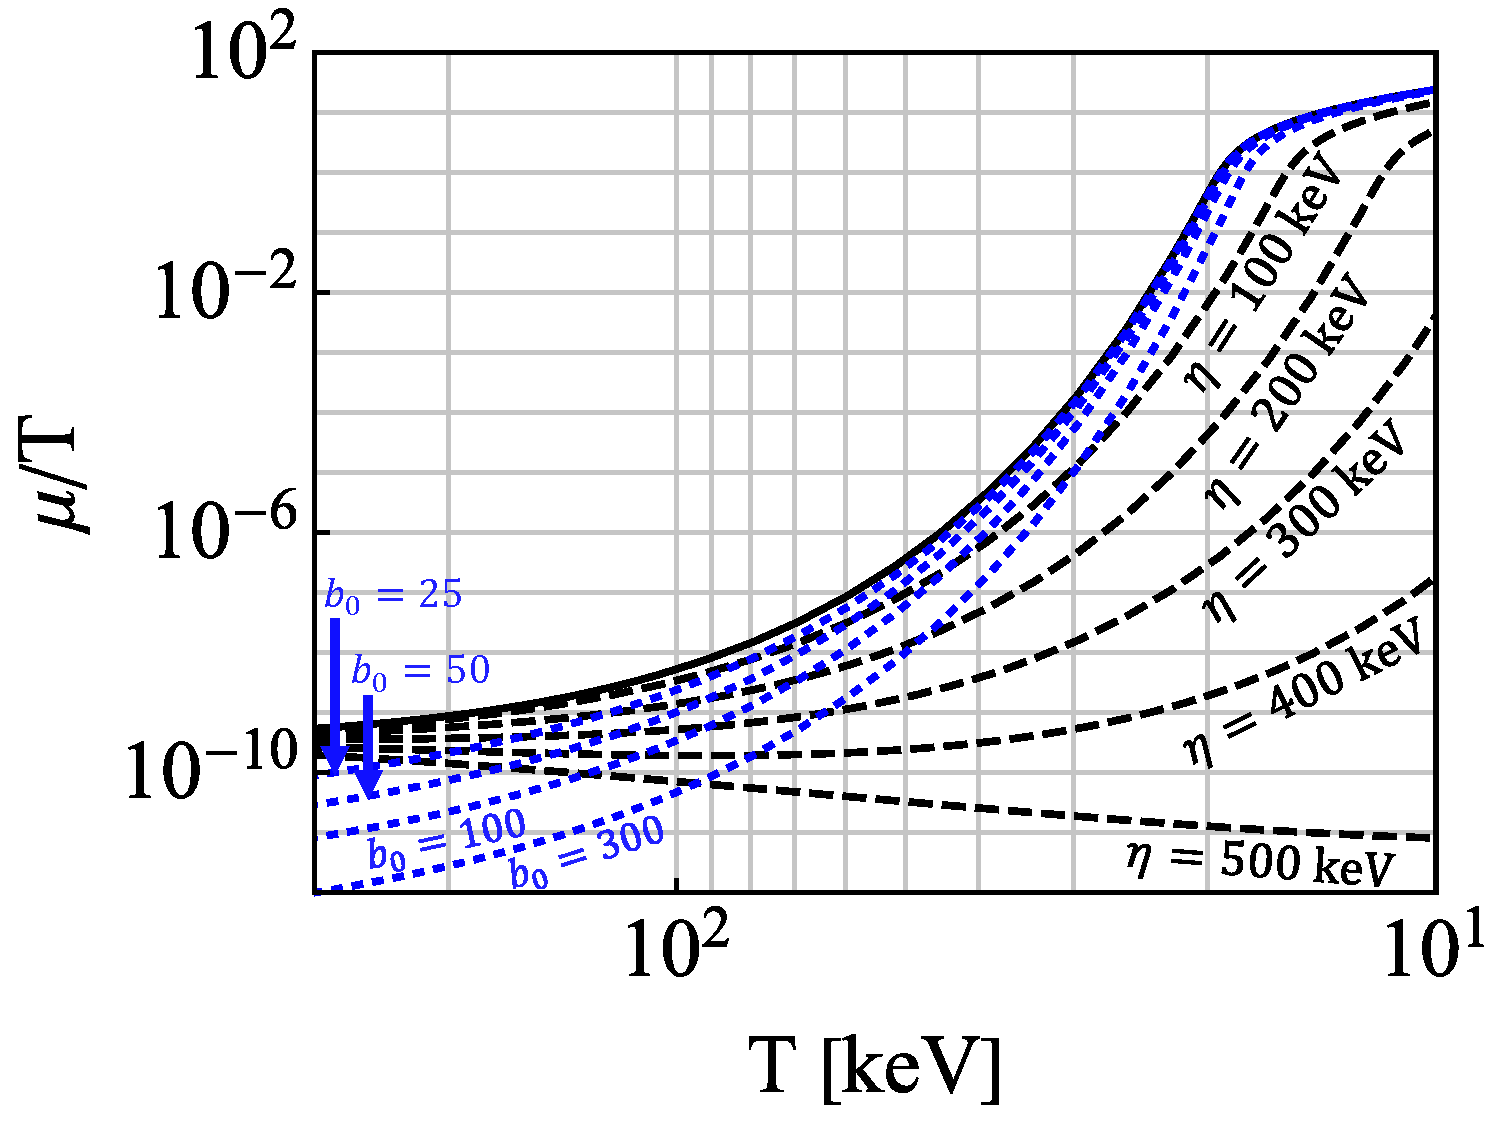
\includegraphics[clip, trim=0.0cm 0.0cm 0.0cm 0.0cm,width=0.95\linewidth]{plots/chap04cosmo/thesis_chempot_fixed.pdf}
 \caption{The chemical potential over temperature $\mu/T$ is plotted as a function of temperature with differing values of spin potential $\eta$ and magnetic scale $b_{0}$.}
 \label{fig:chemicalpotential}
\end{figure}
%%%%%%%%%%%%%%%%%%%%%%%%%%%%%%%%%%%%%%%

\req{chem} simplifies if there is no external magnetic field $b_{0}=0$ into
\begin{align}
    \label{simpchem:1}
    \sinh\frac{\mu}{T}=n_{p}\frac{\pi^{2}}{T^{3}}\left[2\cosh\frac{\eta}{T}\left(\frac{m_{e}}{T}\right)^{2}K_{2}\left(\frac{m_{e}}{T}\right)\right]^{-1}\,.
\end{align}

In \rf{fig:chemicalpotential} we plot the chemical potential $\mu/T$ in \req{chem} and \req{simpchem:1} which characterizes the importance of the charged lepton asymmetry as a function of temperature. Since the baryon (and thus charged lepton) asymmetry remains fixed, the suppression of $\mu/T$ at high temperatures indicates a large pair density which is seen explicitly in \rf{fig:densityratio}. The black line corresponds to the $b_{0}=0$ and $\eta=0$ case. 

The para-diamagnetic contribution from \req{spinorbit} does not appreciably influence $\mu/T$ until the magnetic scales involved become incredibly large well outside the observational bounds defined in \req{igmf} and \req{tbscale} as seen by the dotted blue curves of various large values $b_{0}=\{25,\ 50,\ 100,\ 300\}$. The chemical potential is also insensitive to forcing by the spin potential until $\eta$ reaches a significant fraction of the electron mass $m_{e}$ in size. The chemical potential for large values of spin potential $\eta=\{100,\ 200,\ 300,\ 400,\ 500\}\,\keV$ are also plotted as dashed black lines with $b_{0}=0$.

It is interesting to note that there are crossing points where a given chemical potential can be described as either an imbalance in spin-polarization or presence of external magnetic field. While spin potential suppresses the chemical potential at low temperatures, external magnetic fields only suppress the chemical potential at high temperatures.

The profound insensitivity of the chemical potential to these parameters justifies the use of the free particle chemical potential (black line) in the ranges of magnetic field strength considered for cosmology. Mathematically this can be understood as $\xi$ and $b_{0}$ act as small corrections in the denominator of \req{chem} if expanded in powers of these two parameters.

%%%%%%%%%%%%%%%%%%%%%%%%%%%%%%%%%%%%%%%
\section{Relativistic paramagnetism of electron-positron gas}
\label{sec:magnetization}
%%%%%%%%%%%%%%%%%%%%%%%%%%%%%%%%%%%%%%%
\noindent The total magnetic flux within a region of space can be written as the sum of external fields and the magnetization of the medium via
\begin{align}
 \label{totalmag}
 {B}_\mathrm{total} = {B} + \mathcal{M}\,.
\end{align}
For the simplest mediums without ferromagnetic or hysteresis considerations, the relationship can be parameterized by the susceptibility $\chi$ of the medium as
\begin{align}
 \label{susceptibility}
 {B}_\mathrm{total} = (1+\chi){B}\,,\qquad \mathcal{M} = \chi{B}\,,\qquad \chi\equiv\frac{\partial\mathcal{M}}{\partial{B}}\,,
\end{align}
with the possibility of both paramagnetic materials $(\chi>1)$ and diamagnetic materials $(\chi<1)$. The $e^{+}e^{-}$ plasma however does not so neatly fit in either category as given by \req{spin} and \req{spinorbit}. In general, the susceptibility of the gas will itself be a field dependant quantity.

In our analysis, the external magnetic field always appears within the context of the magnetic scale $b_{0}$, therefore we can introduce the change of variables
\begin{align}
 \frac{\partial b_{0}}{\partial{B}}=\frac{e}{T^{2}}\,.
\end{align}
The magnetization of the $e^{+}e^{-}$ plasma described by the partition function in \req{boltzmann} can then be written as
\begin{align}
 \label{defmagetization}
 \mathcal{M}\equiv\frac{T}{V}\frac{\partial}{\partial{B}}\ln{\mathcal{Z}_{e^{+}e^{-}}} = \frac{T}{V}\left(\frac{\partial b_{0}}{\partial{B}}\right)\frac{\partial}{\partial b_{0}}\ln{\mathcal{Z}_{e^{+}e^{-}}}\,,
\end{align}
Magnetization arising from other components in the cosmic gas (protons, neutrinos, etc.) could in principle also be included. Localized inhomogeneities of matter evolution are often non-trivial and generally be solved numerically using magneto-hydrodynamics (MHD)~\cite{melrose2008quantum,Vazza:2017qge,Vachaspati:2020blt} or with a suitable Boltzmann-Vlasov transport equation. An extension of our work would be to embed magnetization into transport theory~\cite{Formanek:2021blc}. In the context of MHD, primordial magnetogenesis from fluid flows in the electron-positron epoch was considered in~\cite{Gopal:2004ut,Perrone:2021srr}.

We introduce dimensionless units for magnetization ${\mathfrak M}$ by defining the critical field strength
\begin{align}
 {B}_{C}\equiv\frac{m_{e}^{2}}{e}\,,\qquad{\mathfrak M}\equiv\frac{\mathcal{M}}{{B}_{C}}\,.
\end{align}
The scale ${B}_{C}$ is where electromagnetism is expected to become subject to non-linear effects, though luckily in our regime of interest, electrodynamics should be linear. We note however that the upper bounds of IGMFs in \req{igmf} (with $b_{0}=10^{-3}$; see \req{tbscale}) brings us to within $1\%$ of that limit for the external field strength in the temperature range considered.

The total magnetization ${\mathfrak M}$ can be broken into the sum of magnetic moment parallel ${\mathfrak M}_{+}$ and magnetic moment anti-parallel ${\mathfrak M}_{-}$ contributions
\begin{align}
\label{g2mag}
{\mathfrak M}={\mathfrak M}_{+}+{\mathfrak M}_{-}\,.
\end{align}
We note that the expression for the magnetization simplifies significantly for $g\!=\!2$ which is the `natural' gyro-magnetic factor~\cite{Evans:2022fsu,Rafelski:2022bsv} for Dirac particles. For illustration, the $g\!=\!2$ magnetization from \req{defmagetization} is then
\begin{align}
 \label{g2magplus}
 {\mathfrak M}_{+}&=\frac{e^{2}}{\pi^{2}}\frac{T^{2}}{m_{e}^{2}}\xi\cosh{\frac{\mu}{T}}\left[\frac{1}{2}x_{+}K_{1}(x_{+})+\frac{b_{0}}{6}K_{0}(x_{+})\right]\,,\\
 \label{g2magminus}
 -{\mathfrak M}_{-}&=\frac{e^{2}}{\pi^{2}}\frac{T^{2}}{m_{e}^{2}}\xi^{-1}\cosh{\frac{\mu}{T}}
 \left[\left(\frac{1}{2}+\frac{b_{0}^{2}}{12x_{-}^{2}}\right)x_{-}K_{1}(x_{-})+\frac{b_{0}}{3}K_{0}(x_{-})\right]\,,\\
 x_{+}&=\frac{m_{e}}{T}\,,\qquad
 x_{-}=\sqrt{\frac{m_{e}^{2}}{T^{2}}+2b_{0}}\,.
\end{align}
As the $g$-factor of the electron is only slightly above two at $g\simeq2.00232$~\cite{Tiesinga:2021myr}, the above two expressions for ${\mathfrak M}_{+}$ and ${\mathfrak M}_{-}$ are only modified by a small amount because of anomalous magnetic moment (AMM) and would be otherwise invisible on our figures.

%%%%%%%%%%%%%%%%%%%%%%%%%%%%%%%%%%%%%%%
\subsection{Evolution of electron-positron magnetization}
\label{sec:paramagnetism}
%%%%%%%%%%%%%%%%%%%%%%%%%%%%%%%%%%%%%%%
\noindent In \rf{fig:magnet}, we plot the magnetization as given by \req{g2magplus} and \req{g2magminus} with the spin potential set to unity $\xi=1$. The lower (solid red) and upper (solid blue) bounds for cosmic magnetic scale $b_{0}$ are included. The external magnetic field strength ${B}/{B}_{C}$ is also plotted for lower (dotted red) and upper (dotted blue) bounds. Since the derivative of the partition function governing magnetization may manifest differences between Fermi-Dirac and the here used Boltzmann limit more acutely, out of abundance of caution, we indicate extrapolation outside the domain of validity of the Boltzmann limit with dashes.

%%%%%%%%%%%%%%%%%%%%%%%%%%%%%%%%%%%%%%%
\begin{figure}[ht]
 \centering
 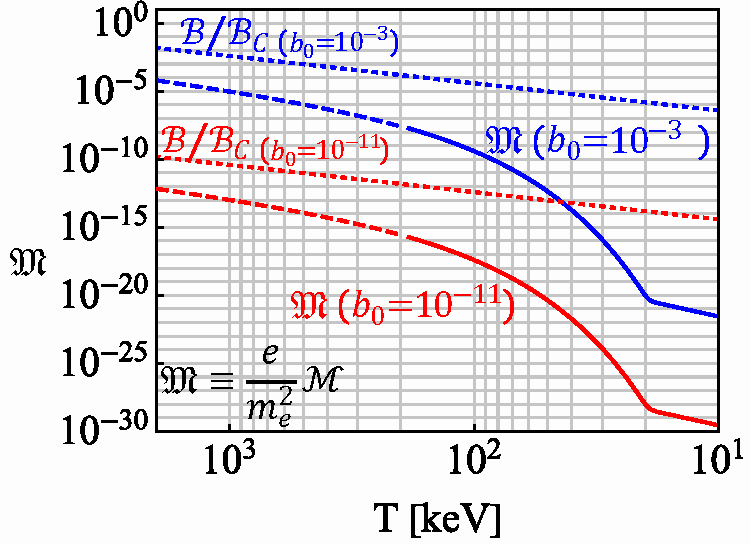
\includegraphics[width=0.95\linewidth]{plots/chap04cosmo/thesis_mag.pdf}
 \caption{The magnetization ${\mathfrak M}$, with $g\!=\!2$, of the primordial $e^{+}e^{-}$ plasma is plotted as a function of temperature. Figure made in collaboration with Cheng Tao Yang.}
 \label{fig:magnet} 
\end{figure}
%%%%%%%%%%%%%%%%%%%%%%%%%%%%%%%%%%%%%%%

We see in \rf{fig:magnet} that the $e^{+}e^{-}$ plasma is overall paramagnetic and yields a positive overall magnetization which is contrary to the traditional assumption that matter-antimatter plasma lack significant magnetic responses of their own in the bulk. With that said, the magnetization never exceeds the external field under the parameters considered which shows a lack of ferromagnetic behavior. 

The large abundance of pairs causes the smallness of the chemical potential seen in~\rf{fig:chemicalpotential} at high temperatures. As the universe expands and temperature decreases, there is a rapid decrease of the density $n_{e^{\pm}}$ of $e^{+}e^{-}$ pairs. This is the primary the cause of the rapid paramagnetic decrease seen in \rf{fig:magnet} above $T\!=\!21\keV$. At lower temperatures $T<21\keV$ there remains a small electron excess (see~\rf{fig:densityratio}) needed to neutralize proton charge. These excess electrons then govern the residual magnetization and dilutes with cosmic expansion.

An interesting feature of \rf{fig:magnet} is that the magnetization in the full temperature range increases as a function of temperature. This is contrary to Curie's law~\cite{greiner2012thermodynamics} which stipulates that paramagnetic susceptibility of a laboratory material is inversely proportional to temperature. However, Curie's law applies to systems with fixed number of particles which is not true in our situation; see \rsec{sec:perlepton}.

A further consideration is possible hysteresis as the $e^{+}e^{-}$ density drops with temperature. It is not immediately obvious the gas's magnetization should simply `degauss' so rapidly without further consequence. If the very large paramagnetic susceptibility present for $T\simeq m_{e}$ is the origin of an overall magnetization of the plasma, the conservation of magnetic flux through the comoving surface ensures that the initial residual magnetization is preserved at a lower temperature by Faraday induced kinetic flow processes however our model presented here cannot account for such effects.

Early universe conditions may also apply to some extreme stellar objects with rapid change in $n_{e^{\pm}}$ with temperatures above $T\!=\!21\keV$. Production and annihilation of $e^{+}e^{-}$ plasmas is also predicted around compact stellar objects~\cite{Ruffini:2009hg,Ruffini:2012it} potentially as a source of gamma-ray bursts.

%%%%%%%%%%%%%%%%%%%%%%%%%%%%%%%%%%%%%%%
\subsection{Dependency on g-factor}
\label{sec:gfac}
%%%%%%%%%%%%%%%%%%%%%%%%%%%%%%%%%%%%%%%

\noindent As discussed at the end of \rsec{sec:magnetization}, the AMM of $e^{+}e^{-}$ is not relevant in the present model. However out of academic interest, it is valuable to consider how magnetization is effected by changing the $g$-factor significantly.

%%%%%%%%%%%%%%%%%%%%%%%%%%%%%%%%%%%%%%%
\begin{figure}[ht]
 \centering
 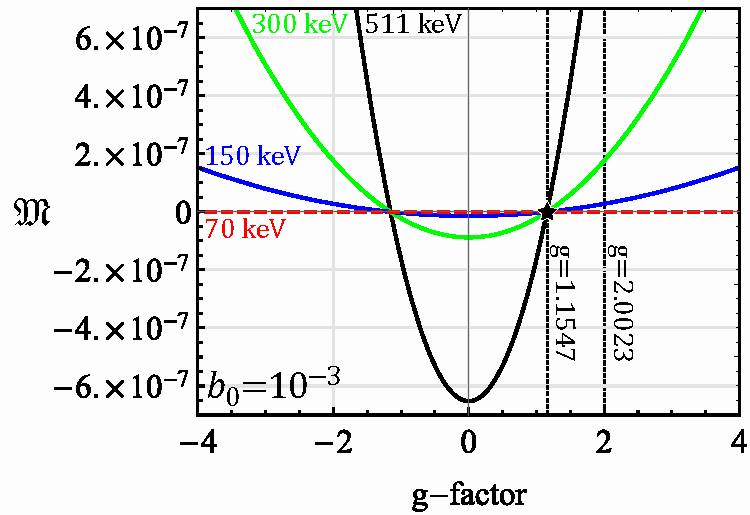
\includegraphics[width=0.95\textwidth]{plots/chap04cosmo/thesis_gfac.pdf}
 \caption{The magnetization $\mathfrak M$ as a function of $g$-factor plotted for several temperatures with magnetic scale $b_{0}=10^{-3}$ and polarization fugacity $\xi=1$.}
 \label{fig:gfac} 
\end{figure}
%%%%%%%%%%%%%%%%%%%%%%%%%%%%%%%%%%%%%%%

The influence of AMM would be more relevant for the magnetization of baryon gasses since the $g$-factor for protons $(g\approx5.6)$ and neutrons $(g\approx3.8)$ are substantially different from $g\!=\!2$. The influence of AMM on the magnetization of thermal systems with large baryon content (neutron stars, magnetars, hypothetical bose stars, etc.) is therefore also of interest~\cite{Ferrer:2019xlr,Ferrer:2023pgq}.

\req{g2magplus} and \req{g2magminus} with arbitrary $g$ reintroduced is given by
\begin{gather}
\label{arbg:1}
{\mathfrak M}=\frac{e^{2}}{\pi^{2}}\frac{T^{2}}{m_{e}^{2}}\sum_{s'}^{\pm1}\xi_{s'}\cosh{\frac{\mu}{T}}
\left[C^{1}_{s'}(x_{s'})K_{1}(x_{s'})+C^{0}_{s'}K_{0}(x_{s'})\right]\,,\\
\label{arbg:2}
C^{1}_{s'}(x_{\pm}) = \left[\frac{1}{2}-\left(\frac{1}{2}-\frac{g}{4}s'\right)\left(1+\frac{b^2_0}{12x^{2}_{s'}}\right)\right]x_{s'}\,,\qquad
C^{0}_{s'} = \left[\frac{1}{6}-\left(\frac{1}{4}-\frac{g}{8}s'\right)\right]b_0\,,
\end{gather}
where $x_{s'}$ was previously defined in \req{xfunc}.

In \rf{fig:gfac}, we plot the magnetization as a function of $g$-factor between $4>g>-4$ for temperatures $T\!=\!\{511,\ 300,\ 150,\ 70\}\keV$. We find that the magnetization is sensitive to the value of AMM revealing a transition point between paramagnetic $({\mathfrak M}>0)$ and diamagnetic gasses $({\mathfrak M}<0)$. Curiously, the transition point was numerically determined to be around $g\simeq1.1547$ in the limit $b_{0}\rightarrow0$. The exact position of this transition point however was found to be both temperature and $b_{0}$ sensitive, though it moved little in the ranges considered.

It is not surprising for there to be a transition between diamagnetism and paramagnetism given that the partition function (see \req{spin} and \req{spinorbit}) contained elements of both. With that said, the transition point presented at $g\approx1.15$ should not be taken as exact because of the approximations used to obtain the above results. 

It is likely that the exact transition point has been altered by our taking of the Boltzmann approximation and Euler-Maclaurin integration steps. It is known that the Klein-Gordon-Pauli solutions to the Landau problem in \req{cosmokgp} have periodic behavior~\cite{Steinmetz:2018ryf,Evans:2022fsu,Rafelski:2022bsv} for $|g|=k/2$ (where $k\in1,2,3\ldots$).

These integer and half-integer points represent when the two Landau towers of orbital levels match up exactly. Therefore, we propose a more natural transition between the spinless diamagnetic gas of $g=0$ and a paramagnetic gas is $g=1$. A more careful analysis is required to confirm this, but that our numerical value is close to unity is suggestive.

%%%%%%%%%%%%%%%%%%%%%%%%%%%%%%%%%%%%%%%
\subsection{Magnetization per lepton}
\label{sec:perlepton}
%%%%%%%%%%%%%%%%%%%%%%%%%%%%%%%%%%%%%%%
\noindent Despite the relatively large magnetization seen in \rf{fig:magnet}, the average contribution per lepton is only a small fraction of its overall magnetic moment indicating the magnetization is only loosely organized. Specifically, the magnetization regime we are in is described by
\begin{align}
 \label{fractionalmagnetization}
 \mathcal{M}\ll\mu_{B}\frac{N_{e^{+}}+N_{e^{-}}}{V}\,,\qquad\mu_{B}\equiv\frac{e}{2m_{e}}\,,
\end{align}
where $\mu_{B}$ is the Bohr magneton and $N=nV$ is the total particle number in the proper volume V. To better demonstrate that the plasma is only weakly magnetized, we define the average magnetic moment per lepton given by along the field ($z$-direction) axis as
\begin{align}
 \label{momentperlepton}
 \vert\vec{m}\vert_{z}\equiv\frac{\mathcal{M}}{n_{e^{-}}+n_{e^{+}}}\,,\qquad\vert\vec{m}\vert_{x}=\vert\vec{m}\vert_{y}=0\,.
\end{align}
Statistically, we expect the transverse expectation values to be zero. We emphasize here that despite $|\vec{m}|_{z}$ being nonzero, this doesn't indicate a nonzero spin angular momentum as our plasma is nearly matter-antimatter symmetric. The quantity defined in \req{momentperlepton} gives us an insight into the microscopic response of the plasma.

%%%%%%%%%%%%%%%%%%%%%%%%%%%%%%%%%%%%%%%
\begin{figure}[ht]
 \centering
 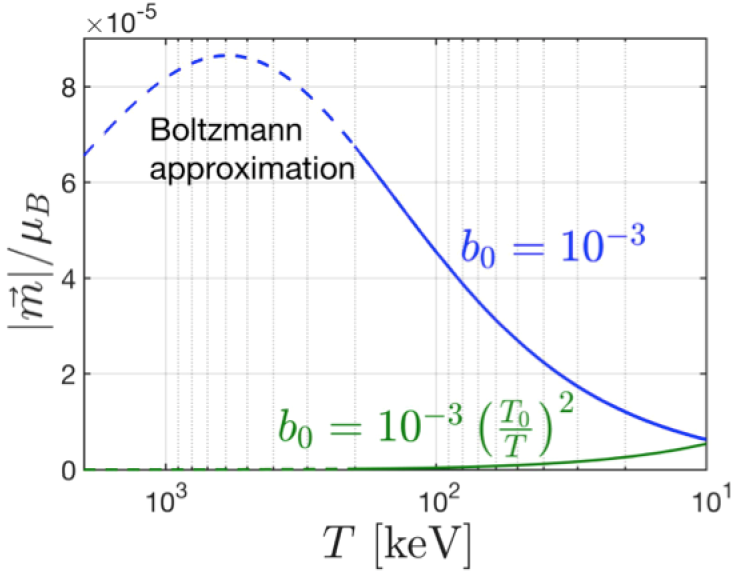
\includegraphics[clip, trim=0.0cm 0.0cm 0.0cm 0.0cm,width=0.95\textwidth]{plots/chap04cosmo/thesis_perlepton.png}
 \caption{The magnetic moment per lepton $\vert\vec{m}\vert_{z}$ along the field axis as a function of temperature. Figure made in collaboration with Cheng Tao Yang.}
 \label{fig:momentperlepton}
\end{figure}
%%%%%%%%%%%%%%%%%%%%%%%%%%%%%%%%%%%%%%%

The average magnetic moment $\vert\vec{m}\vert_{z}$ defined in \req{momentperlepton} is plotted in \rf{fig:momentperlepton} which displays how essential the external field is on the `per lepton' magnetization. The $b_{0}=10^{-3}$ case (blue curve) is plotted in the Boltzmann approximation. The dashed lines indicate where this approximation is only qualitatively correct. For illustration, a constant magnetic field case (solid green line) with a comoving reference value chosen at temperature $T_{0}=10\keV$ is also plotted.

If the field strength is held constant, then the average magnetic moment per lepton is suppressed at higher temperatures as expected for magnetization satisfying Curie's law. The difference in \rf{fig:momentperlepton} between the non-constant (blue solid curve) case and the constant field (solid green curve) case demonstrates the importance of the conservation of primordial magnetic flux in the plasma, required by \req{bscale}. While not shown, if \rf{fig:momentperlepton} was extended to lower temperatures, the magnetization per lepton of the constant field case would be greater than the non-constant case which agrees with our intuition that magnetization is easier to achieve at lower temperatures. This feature again highlights the importance of flux conservation in the system and the uniqueness of the primordial cosmic environment.

%%%%%%%%%%%%%%%%%%%%%%%%%%%%%%%%%%%%%%%
\section{Polarization potential and ferromagnetism}
\label{sec:ferro}
%%%%%%%%%%%%%%%%%%%%%%%%%%%%%%%%%%%%%%%
\noindent Up to this point, we have neglected the impact that a nonzero spin potential $\eta\neq0$ (and thus $\xi\neq1$) would have on the primordial $e^{+}e^{-}$ plasma magnetization. In the limit that $(m_{e}/T)^2\gg b_0$ the magnetization given in \req{arbg:1} and \req{arbg:2} is entirely controlled by the spin fugacity $\xi$ asymmetry generated by the spin potential $\eta$ yielding up to first order $\mathcal{O}(b_{0})$ in magnetic scale
\begin{multline}
 \label{ferro}
 \lim_{m_{e}^{2}/T^{2}\gg b_0}{\mathfrak M}=\frac{g}{2}\frac{e^{2}}{\pi^{2}}\frac{T^{2}}{m_{e}^{2}}\sinh{\frac{\eta}{T}}\cosh{\frac{\mu}{T}}\left[\frac{m_{e}}{T}K_{1}\left(\frac{m_{e}}{T}\right)\right]\\
 +b_{0}\left(g^{2}-\frac{4}{3}\right)\frac{e^{2}}{8\pi^{2}}\frac{T^{2}}{m_{e}^{2}}\cosh{\frac{\eta}{T}}\cosh{\frac{\mu}{T}}K_{0}\left(\frac{m_{e}}{T}\right)
 +\mathcal{O}\left(b_{0}^{2}\right)
\end{multline}

Given \req{ferro}, we can understand the spin potential as a kind of `ferromagnetic' influence on the primordial gas which allows for magnetization even in the absence of external magnetic fields. This interpretation is reinforced by the fact the leading coefficient is $g/2$.

We suggest that a variety of physics could produce a small nonzero $\eta$ within a domain of the gas. Such asymmetries could also originate statistically as while the expectation value of free gas polarization is zero, the variance is likely not.

As $\sinh{\eta/T}$ is an odd function, the sign of $\eta$ also controls the alignment of the magnetization. In the high temperature limit \req{ferro} with strictly $b_{0}=0$ assumes a form of to lowest order for brevity
\begin{align}
 \label{hiTferro}
 \lim_{m_{e}/T\rightarrow0}{\mathfrak M}\vert_{b_{0}=0}=\frac{g}{2}\frac{e^{2}}{\pi^{2}}\frac{T^{2}}{m_{e}^{2}}\frac{\eta}{T}\,,
\end{align}

While the limit in \req{hiTferro} was calculated in only the Boltzmann limit, it is noteworthy that the high temperature (and $m\rightarrow0$) limit of Fermi-Dirac distributions only differs from the Boltzmann result by a proportionality factor. 

The natural scale of the $e^{+}e^{-}$ magnetization with only a small spin fugacity ($\eta<1\eV$) fits easily within the bounds of the predicted magnetization during this era if the IGMF measured today was of primordial origin. The reason for this is that the magnetization seen in \req{g2magplus}, \req{g2magminus} and \req{ferro} are scaled by $\alpha{B}_{C}$ where $\alpha$ is the fine structure constant.

%%%%%%%%%%%%%%%%%%%%%%%%%%%%%%%%%%%%%%%
\subsection{Hypothesis of ferromagnetic self-magnetization}
\label{sec:self}
%%%%%%%%%%%%%%%%%%%%%%%%%%%%%%%%%%%%%%%
\noindent One exploratory model we propose is to fix the spin polarization asymmetry, described in \req{spotential}, to generate a homogeneous magnetic field which dissipates as the universe cools down. In this model, there is no external primordial magnetic field $({B}_\mathrm{PMF}=0)$ generated by some unrelated physics, but rather the $e^{+}e^{-}$ plasma itself is responsible for the field by virtue of spin polarization.

%%%%%%%%%%%%%%%%%%%%%%%%%%%%%%%%%%%%%%%
\begin{figure}[ht]
 \centering
 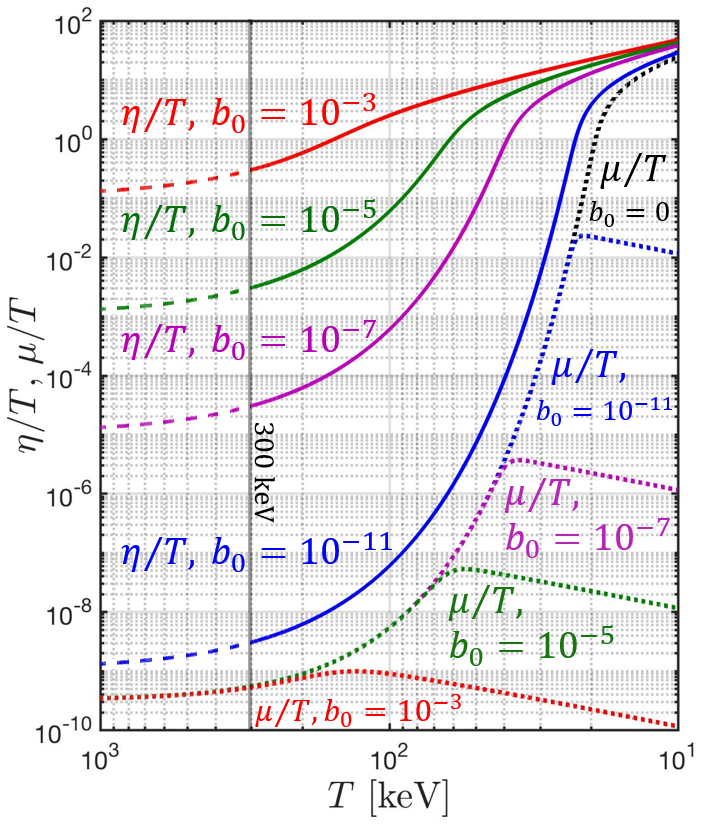
\includegraphics[width=0.5\textwidth]{plots/chap04cosmo/Spinchemical_03.png}
 \caption{The spin potential $\eta$ and chemical potential $\mu$ are plotted under the assumption of self-magnetization through a nonzero spin polarization in bulk of the plasma. Figure made in collaboration with Cheng Tao Yang.}
 \label{fig:self} 
\end{figure}
%%%%%%%%%%%%%%%%%%%%%%%%%%%%%%%%%%%%%%%

This would obey the following assumption of
\begin{align}
 \label{selfmag}
 {\mathfrak M}(b_{0})=\frac{\mathcal{M}(b_0)}{{B}_{C}}\longleftrightarrow\frac{B}{{B}_{C}}=b_{0}\frac{T^{2}}{m_{e}^{2}}\,,
\end{align}
which sets the total magnetization as a function of itself. The spin polarization described by $\eta\rightarrow\eta(b_{0},T)$ then becomes a fixed function of the temperature and magnetic scale. The underlying assumption would be the preservation of the homogeneous field would be maintained by scattering within the gas (as it is still in thermal equilibrium) modulating the polarization to conserve total magnetic flux.

The result of the self-magnetization assumption in \req{selfmag} for the potentials is plotted in \rf{fig:self}. The solid lines indicate the curves for $\eta/T$ for differing values of $b_{0}=\{10^{-11},\ 10^{-7},\ 10^{-5},\ 10^{-3}\}$ which become dashed above $T\!=\!300\keV$ to indicate that the Boltzmann approximation is no longer appropriate though the general trend should remain unchanged.

%%%%%%%%%%%%%%%%%%%%%%%%%%%%%%%%%%%%%%%
\begin{figure}[ht]
 \centering
 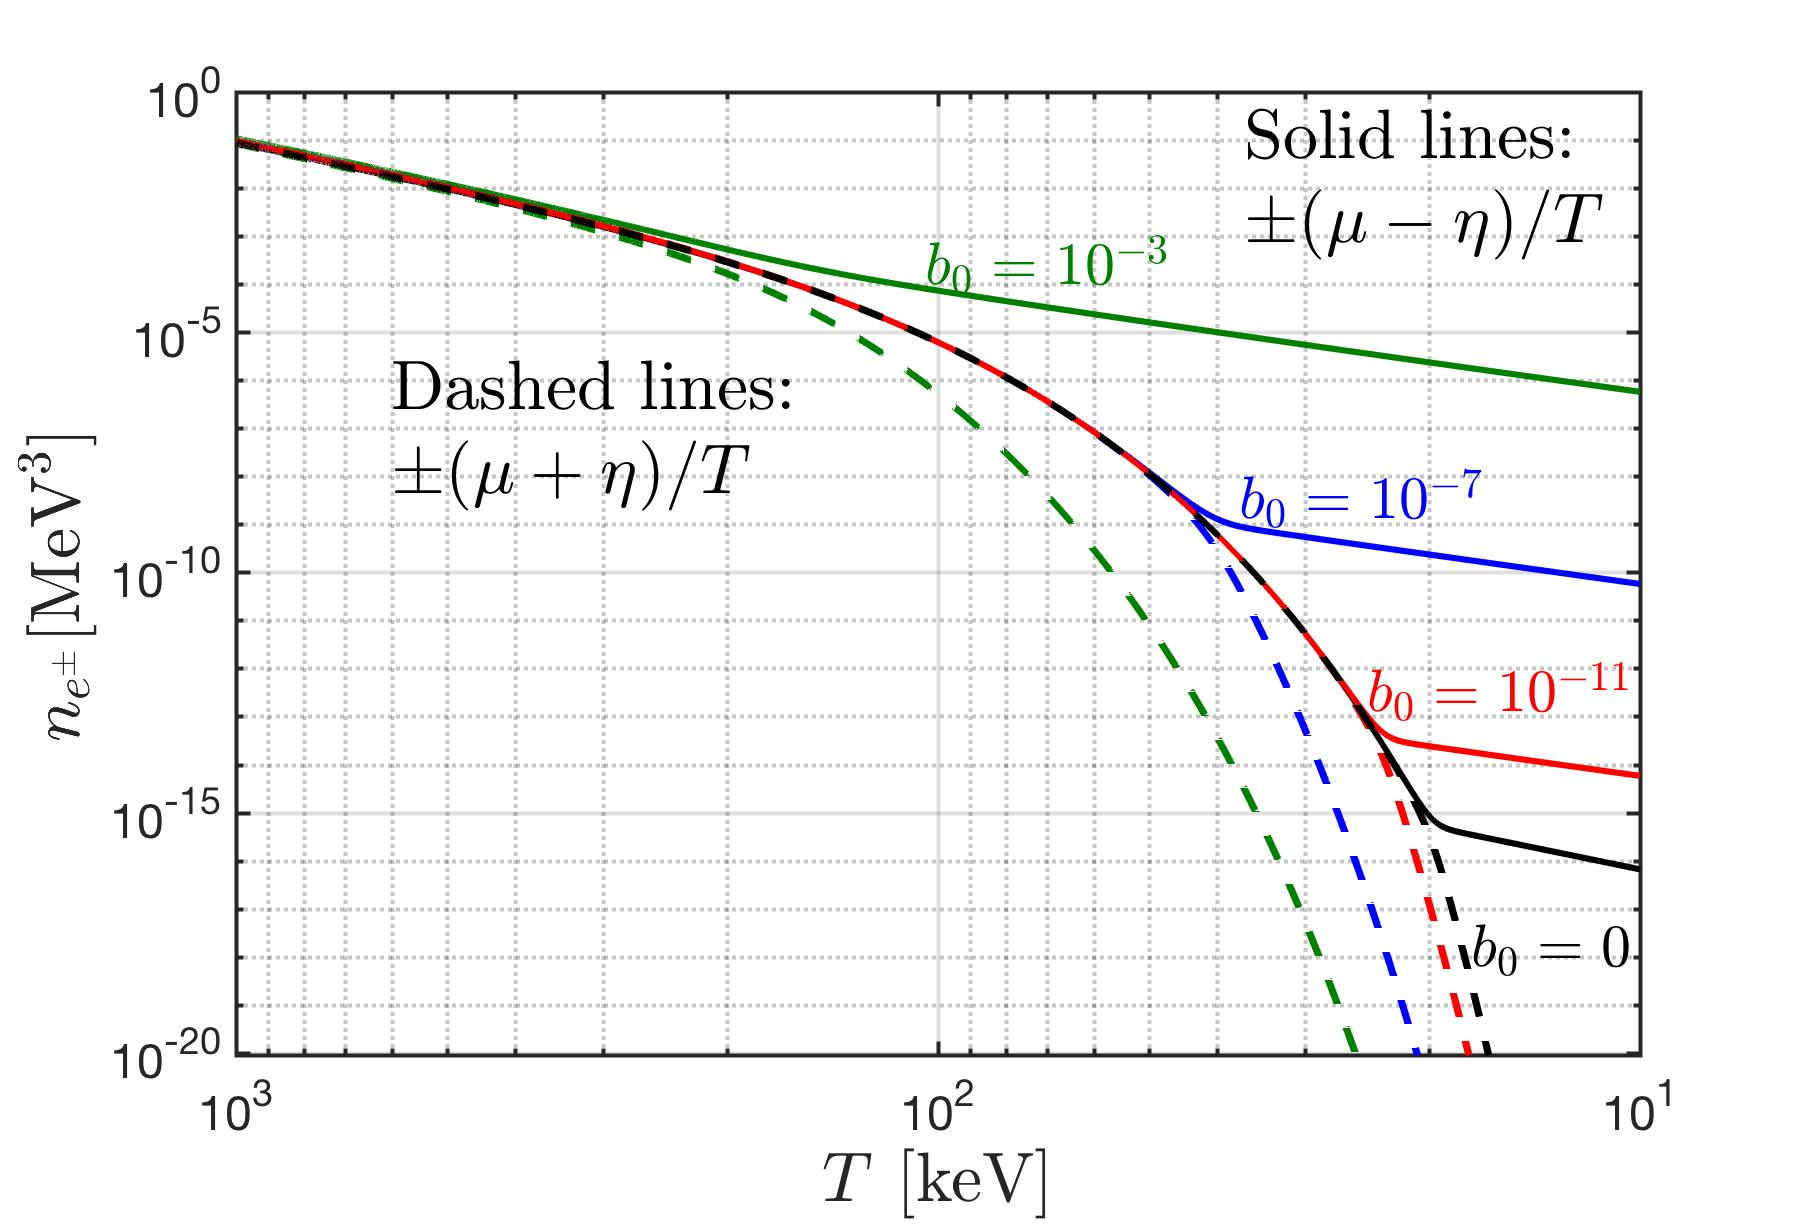
\includegraphics[width=0.95\textwidth]{plots/chap04cosmo/ElectronDensity_SpinChemicalPotential004.jpg}
 \caption{The number density $n_{e^{\pm}}$ of polarized electrons and positrons under the self-magnetization model for differing values of $b_{0}$. Figure courtesy of Cheng Tao Yang.}
 \label{fig:polarswap} 
\end{figure}
%%%%%%%%%%%%%%%%%%%%%%%%%%%%%%%%%%%%%%%

The dotted lines are the curves for the chemical potential $\mu/T$. At high temperatures we see that a relatively small $\eta/T$ is needed to produce magnetization owing to the large densities present. \rf{fig:self} also shows that the chemical potential does not deviate from the free particle case until the spin polarization becomes sufficiently high which indicates that this form of self-magnetization would require the annihilation of positrons to be incomplete even at lower temperatures.

This is seen explicitly in~\rf{fig:polarswap} where we plot the numerical density of particles as a function of temperature for spin aligned $(+\eta)$ and spin anti-aligned $(-\eta)$ species for both positrons $(-\mu)$ and electrons $(+\mu)$. Various self-magnetization strengths are also plotted to match those seen in~\rf{fig:self}. The nature of $T_{\rm split}$ changes under this model since antimatter and polarization states can be extinguished separately. Positrons persist where there is insufficient electron density to maintain the magnetic flux. Polarization asymmetry therefore appears physical only in the domain where there is a large number of matter-antimatter pairs.

%%%%%%%%%%%%%%%%%%%%%%%%%%%%%%%%%%%%%%%
\subsection{Matter inhomogeneities in the cosmic plasma}
\label{sec:inhomogeneous}
%%%%%%%%%%%%%%%%%%%%%%%%%%%%%%%%%%%%%%%
\noindent In general, an additional physical constraint is required to fully determine $\mu$ and $\eta$ simultaneously as both potentials have mutual dependency (see \rsec{sec:ferro}). We note that spin polarizations are not required to be in balanced within a single species to preserve angular momentum.

The CMB~\cite{Planck:2018vyg} indicates that the early universe was home to domains of slightly higher and lower baryon densities which resulted in the presence of galactic super-clusters, cosmic filaments, and great voids seen today. However, the CMB, as measured today, is blind to the localized inhomogeneities required for gravity to begin galaxy and supermassive black hole formation.

Such acute inhomogeneities distributed like a dust~\cite{Grayson:2023flr} in the plasma would make the proton density sharply and spatially dependant $n_{p}\rightarrow n_{p}(x)$ which would directly affect the potentials $\mu(x)$ and $\eta(x)$ and thus the density of electrons and positrons locally. This suggests that $e^{+}e^{-}$ may play a role in the initial seeding of gravitational collapse. If the plasma were home to such localized magnetic domains, the nonzero local angular momentum within these domains would provide a natural mechanism for the formation of rotating galaxies today.

Recent measurements by the James Webb Space Telescope (JWST)~\cite{Yan:2022sxd,adams2023discovery,arrabal2023spectroscopic} indicate that galaxy formation began surprisingly early at large redshift values of $z\gtrsim10$ within the first 500 million years of the universe requiring gravitational collapse to begin in a hotter environment than expected. The observation of supermassive black holes already present~\cite{CEERSTeam:2023qgy} in this same high redshift period (with millions of solar masses) indicates the need for local high density regions in the early universe whose generation is not yet explained and likely need to exist long before the recombination epoch.


\bibliographystyle{spphys}
\bibliography{bibs/birrell-refs,bibs/steinmetz-refs}
%%%%%%%%%%%%%%%%%%%%%%%%
\end{document}
